%%
%% StructWeaver — CHI 2027 Papers submission
%% Built on ACM Primary Article Template (acmart v2.20, 2026/08/16)
%% Official CHI formats: https://chi2027.acm.org/chi-publication-formats/
%% Overleaf: ACM Conference Proceedings Primary Article Template
%%   keep this file as sigconf-authordraft.tex
%%
%% Review / PCS submission (current):
%%   \documentclass[manuscript,review,anonymous]{acmart}
%%
%% After conditional acceptance / TAPS publication-ready:
%%   \documentclass[sigconf]{acmart}
%%
\documentclass[manuscript,review,anonymous]{acmart}
%%
%% \BibTeX command to typeset BibTeX logo in the docs
\AtBeginDocument{%
 \providecommand\BibTeX{{%
 Bib\TeX}}}

%% Rights management information. This information is sent to you
%% when you complete the rights form. These commands have SAMPLE
%% values in them; it is your responsibility as an author to replace
%% the commands and values with those provided to you when you
%% complete the rights form.
\settopmatter{printacmref=false}
%% Rights management information omitted for anonymous review submission.


%%
%% Submission ID.
%% Use this when submitting an article to a sponsored event. You'll
%% receive a unique submission ID from the organizers
%% of the event, and this ID should be used as the parameter to this command.
%%\acmSubmissionID{123-A56-BU3}

%%
%% For managing citations, it is recommended to use bibliography
%% files in BibTeX format.
%%
%% You can then either use BibTeX with the ACM-Reference-Format style,
%% or BibLaTeX with the acmnumeric or acmauthoryear sytles, that include
%% support for advanced citation of software artefact from the
%% biblatex-software package, also separately available on CTAN.
%%
%% Look at the sample-*-biblatex.tex files for templates showcasing
%% the biblatex styles.
%%

%%
%% The majority of ACM publications use numbered citations and
%% references. The command \citestyle{authoryear} switches to the
%% "author year" style.
%%
%% If you are preparing content for an event
%% sponsored by ACM SIGGRAPH, you must use the "author year" style of
%% citations and references.
%% Uncommenting
%% the next command will enable that style.
%%\citestyle{acmauthoryear}


%%
%% end of the preamble, start of the body of the document source.
\usepackage{enumitem}
\usepackage{tabularx}
\usepackage{tikz}
\usepackage{subcaption}
\usepackage{xcolor}
\usepackage{pifont}

\usetikzlibrary{arrows.meta,positioning,fit}
% \newcommand{\highlight}[1]{\textcolor{black}{#1}}
\newcommand{\pcol}[2]{\cellcolor{#1}#2}
% \newcommand{\highlight}[1]{\textcolor{red}{#1}}
\newcommand{\highlight}[1]{#1}
\usepackage{longtable}
\usepackage{booktabs}
\usepackage{array}
\usepackage{colortbl}
\usepackage{multirow}
\usepackage{algorithm}
\usepackage{algpseudocode}
\setlength{\emergencystretch}{1em}
\definecolor{headerbg}{RGB}{230,230,250}
\definecolor{iclbg}{RGB}{255,245,238}
\definecolor{eclbg}{RGB}{240,255,240}
\definecolor{gclbg}{RGB}{240,248,255}
\definecolor{uslbg}{RGB}{250,250,250}
\definecolor{paper1bg}{RGB}{240,248,255}
\definecolor{paper2bg}{RGB}{255,248,240}
\definecolor{paper3bg}{RGB}{248,255,248}
\definecolor{paper4bg}{RGB}{255,248,255}
% , - User color palette , -
\definecolor{p1}{HTML}{F8D7DA} % light pink
\definecolor{p2}{HTML}{D1ECF1} % light cyan
\definecolor{p3}{HTML}{E2D9F3} % light lavender
\definecolor{p4}{HTML}{FFF3CD} % light yellow
\definecolor{p5}{HTML}{FCE5CD} % light orange
\definecolor{p6}{HTML}{D4EDDA} % light green
\definecolor{p7}{HTML}{D6D8FF} % light periwinkle
\definecolor{p8}{HTML}{E8F5E9} % very light green
\definecolor{p9}{HTML}{D0F0F7} % light blue-cyan
\definecolor{p10}{HTML}{E7F5FF} % light blue
\definecolor{p11}{HTML}{EDE7F6} % light purple
\definecolor{p12}{HTML}{F1F8E9} % pale lime
\begin{document}

%%
%% The "title" command has an optional parameter,
%% allowing the author to define a "short title" to be used in page headers.
% \title[When Abstraction Becomes Irreversible]{When Abstraction Becomes Irreversible: Rebuilding Understand--Verify--Re-understand Loops in AI-Assisted Reading}

\title{StructWeaver: Supporting Gist-Verbatim Alignment for Verifiable AI-Assisted Sensemaking}

%%
%% The "author" command and its associated commands are used to define
%% the authors and their affiliations.
%% Of note is the shared affiliation of the first two authors, and the
%% "authornote" and "authornotemark" commands
%% used to denote shared contribution to the research.
\author{Anonymous Author(s)}
\affiliation{%
 \institution{Anonymous Institution}
 \country{Anonymous}}
\email{anonymous@anonymous.com}

%%
%% By default, the full list of authors will be used in the page
%% headers. Often, this list is too long, and will overlap
%% other information printed in the page headers. This command allows
%% the author to define a more concise list
%% of authors' names for this purpose.
\renewcommand{\shortauthors}{Anonymous Author(s)}
%%
%% The abstract is a short summary of the work to be presented in the
%% article.
% \begin{abstract}

% Generative AI makes long-document reading easier by supplying fluent, on-demand gist, yet this fluency creates an abstraction layer that is difficult to traverse back to the source. The problem is not merely that AI-generated gist may be inaccurate, but that once source text is transformed into fluent abstraction, readers lack a stable way to return from gist to the verbatim evidence that produced it. We call this a broken Gist--Verbatim path: a structural failure of reversible alignment, related to but distinct from interpretive misalignment (AI overviews that select different interpretive paths while offering no handles back to source order).

% We contribute Gist--Verbatim alignment, which decomposes AI-generated gist into manipulable units and binds each unit to order-preserving, sentence-level source evidence through embedding-based dynamic-programming alignment. \textit{StructWeaver} instantiates this alignment for conversational single-document reading: it preserves open-ended prompting while making each gist unit, its grounding sentences, and follow-up dialogue co-navigable within a familiar chat-and-PDF workflow.

% Following a formative interview study and a paired within-subjects evaluation ($n=12$), we found that traversable abstractions reconfigured AI-assisted reading from summary consumption toward source grounding. Rather than treating AI outputs as terminal responses, participants repeatedly moved between gist and evidence to inspect AI interpretations, notice omissions, and repair misalignments with author arguments. Verification became embedded in ordinary reading rather than triggered only by explicit doubt, and participants reported that checking source text was easier to perform when abstraction and evidence shared a recoverable path. Participant-level summary quality showed no stable significant system advantage; pooled-triple analyses were annotator-sensitive, suggesting that these process shifts did not come at an obvious cost on headline outcome metrics.
% \end{abstract}


\begin{abstract}
We investigated how readers verify AI-generated interpretations during long-form reading and identified difficulties in maintaining recoverable relationships between AI abstractions and source evidence. We present StructWeaver, an interactive AI-assisted reading system that supports decomposable gist representations, direct Gist--Verbatim traversal, and persistent interpretation paths. A paired within-subjects study with 12 participants showed that StructWeaver shifted AI-assisted reading from repeated summary consumption toward source grounding. Participants used linked evidence to inspect AI interpretations, identify incomplete support, and repair misalignment with author arguments, while reporting lower coordination burden and greater engagement in organizing and integrating information. Our findings highlight reversible abstraction as a design direction for verifiable AI-assisted reading.
\end{abstract}


%%
%% The code below is generated by the tool at http://dl.acm.org/ccs.cfm.
%% Please copy and paste the code instead of the example below.
%%
%%
%% CCS concepts omitted for draft; generate at https://dl.acm.org/ccs/ccs.cfm before camera-ready.
%%\begin{CCSXML}
%%...
%%\end{CCSXML}
%%\ccsdesc[500]{...}

%%
%% Keywords. The author(s) should pick words that accurately describe
%% the work being presented. Separate the keywords with commas.
\keywords{Gist--Verbatim alignment, reversible abstraction, AI-assisted reading, interpretive misalignment, long-form reading, behavioral probe}
%% A "teaser" image appears between the author and affiliation
%% information and the body of the document, and typically spans the
%% page.
\begin{teaserfigure}
 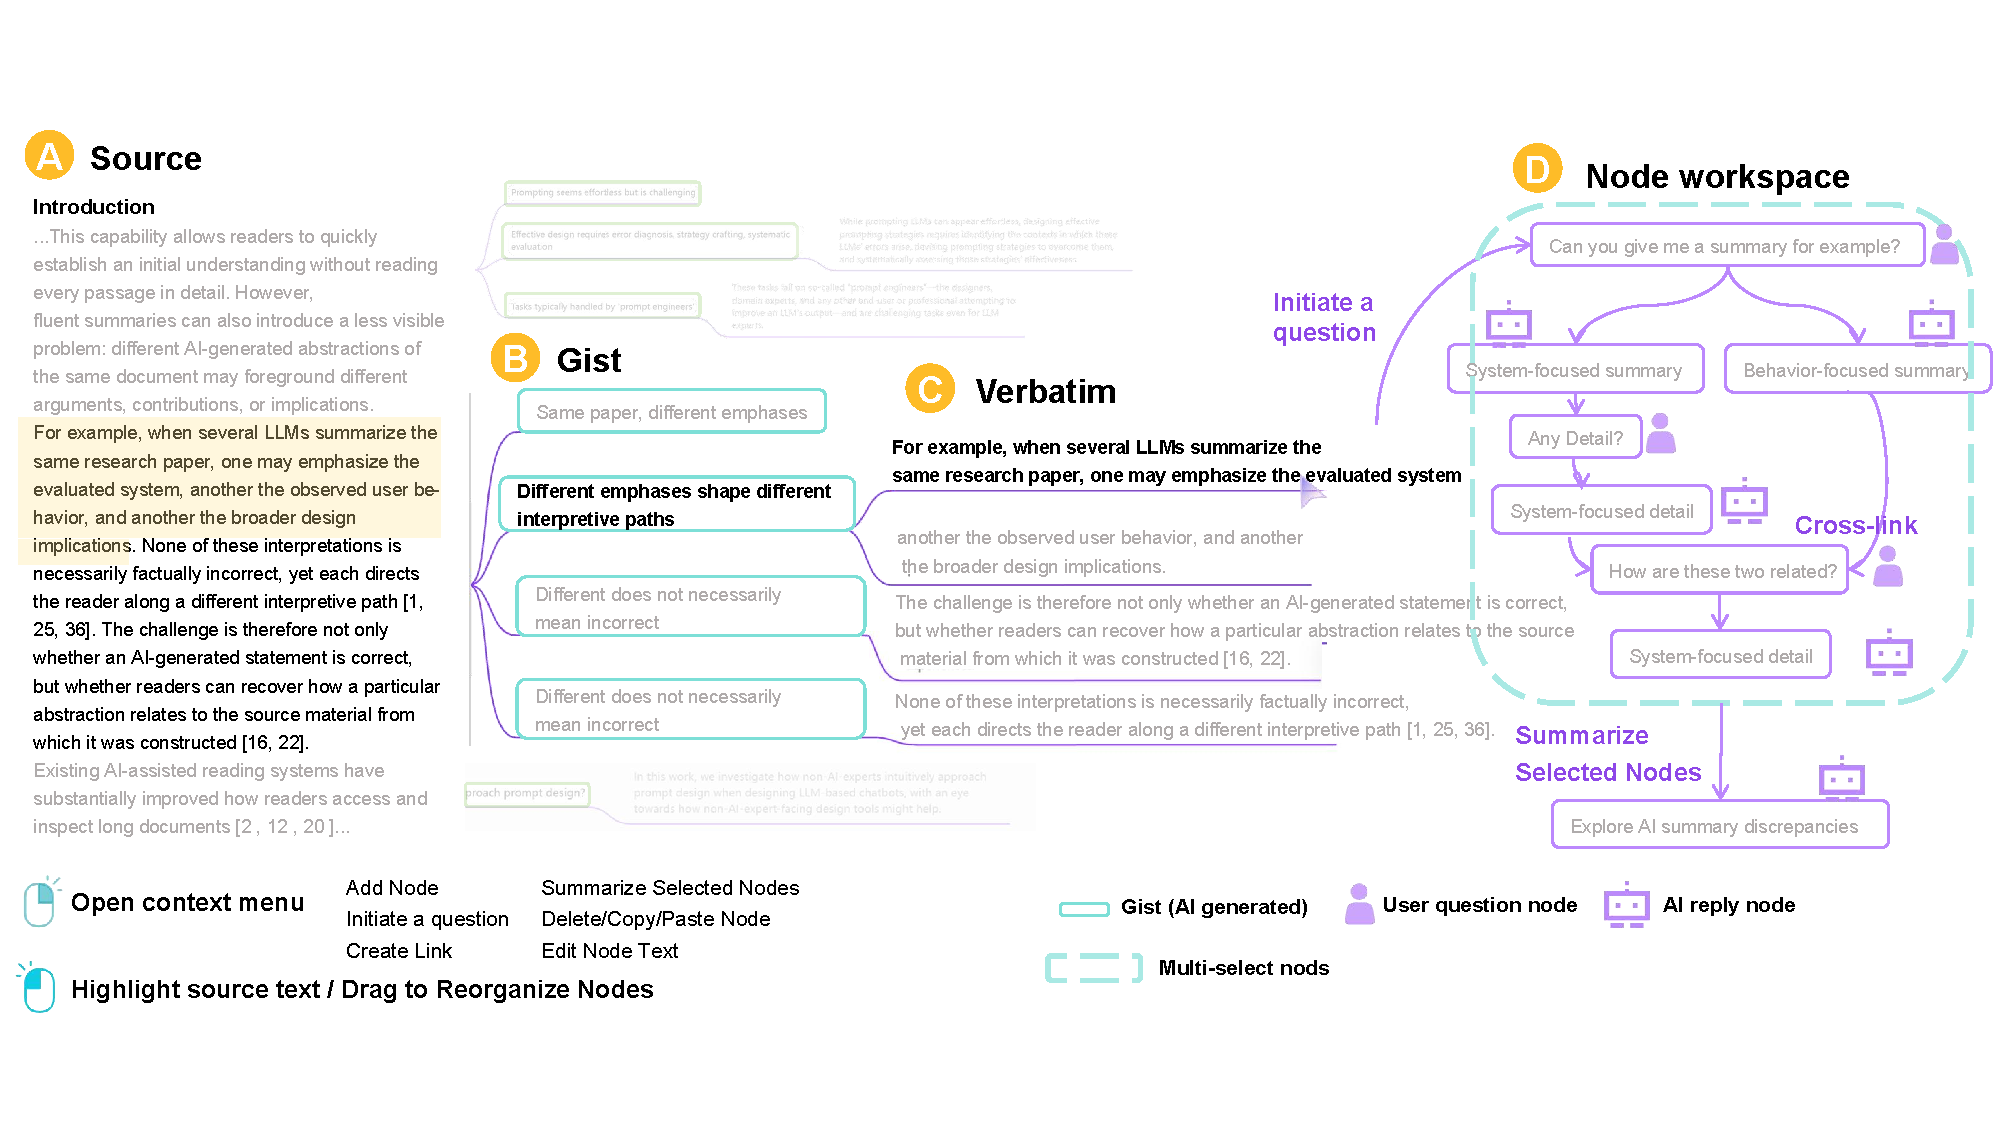
\includegraphics[trim=0 42 0 8, clip, width=\textwidth]{fig/teaser.pdf}
 \caption{StructWeaver supports a reading process from AI-generated gist to source verification to continued questioning. \emph{(1) I ask:} a reader requests an overview from a conventional model. \emph{(2) I open StructWeaver to explore:} the system connects gist nodes to corresponding verbatim evidence and source passages. \emph{(3) I continue the conversation:} follow-up questions attach to the active interpretation branch rather than a global chat, and the reading path grows with exploration.}
 \label{fig:teaser}
\end{teaserfigure}



\maketitle

% \section{Introduction}

% Consider sending Zamfirescu-Pereira et al.'s \textit{Why Johnny Can't Prompt}~\cite{Zamfirescu-Pereira} to different LLMs and asking each for a brief summary. One model emphasizes a no-code chatbot design tool, BotDesigner, and how ten participants with little LLM experience iteratively improved prompts for a cooking-guidance bot. Another foregrounds how non-experts intuitively approach prompt engineering, the difficulties they encounter, and what those findings imply for tools aimed at everyday users. A third stresses that non-experts rarely evaluate prompts systematically, instead transferring human conversational habits into prompt design: over-relying on instructions, resisting examples, and misjudging model comprehension, yielding shallow designs that are hard to keep robust.

% All three summaries read fluently and look as if they reflect the full paper. Yet if we ask what the paper is \emph{really} about: an observation of the prompt-design process? an evaluation of a design tool? or a revelation of everyday users' cognitive limits? The answers diverge. More crucially: if you care about \emph{how conversational habits shape prompt design}, reading only the first or second summary may miss the argument line emphasized in the third, and vice versa. None is obviously wrong, but each imposes a distinct interpretive frame that can steer the reader's attention, expectations, and subsequent judgment of the paper. Classic work on framing shows that equivalent information can yield different impressions depending on how it is presented~\cite{tversky1981framing}; recent studies of LLM-generated summaries and rewrites further show that models introduce framing bias through selective emphasis and omission~\cite{pastorino2025framing,alessa2025quantifying}, with measurable effects on downstream user judgment~\cite{alessa2025quantifying}. Many readers discover only after checking the source that they have lost a contribution they would have wanted to keep.

% Formative interviews (§\ref{sec:formative-implications}) show that readers are not always unwilling to verify, but often struggle to \emph{maintain the path verification requires}. One participant described AI summaries as ``often making sense'' until they tried to compare the AI overview, the author's text, and the storyline they wanted to present: ``the AI's logic, the author's logic, and the logic I wanted to present often did not align.'' Another noted that in the typical chat-plus-PDF split-screen, model replies and paper text appear ``here and there''; aligning claims with evidence between two walls of text turns verification from a natural step in reading into repeated context switching and reconstruction.

% The key risk in AI-assisted reading is not only factual error or hallucination. More common and more insidious is that AI-generated summaries may not be obviously wrong yet already select an interpretive path, emphasizing some contributions, downplaying others, misaligned with the author's argument or the reader's own goal. We call this interpretive misalignment. Verification then is not merely checking whether a claim has a source, but comparing whether three ways of organizing the material can be realigned: how the AI organizes the paper, how the author develops the argument, and how the reader wants to understand and use it.

% Existing workflows struggle to support this alignment. Generative AI offers a flexible, personalized entry point, but it also compresses source text into a fluent, self-contained abstraction that is difficult to traverse back. Even when systems provide finer-grained provenance or evidence links, these signals are typically accessed through additional effort and do not become part of the reader's primary, in-line comprehension process. Readers must pause current reading and launch an extra verification action between overview and source.

% We therefore reformulate the problem as a representation problem: AI-assisted reading needs not only visible evidence, but an entry point that helps readers move naturally into the source text. Readers should be able to move down from AI gist to the author's verbatim evidence and back up into their own interpretive path to continue organizing understanding. Verification should not be an audit after reading, but a natural move in sensemaking.

% Building on this, we present \textit{StructWeaver} (Figure~\ref{fig:teaser}). StructWeaver reconfigures information readers already have: AI-generated gist, author source text, and the reader's own questions and extended understanding. The system decomposes AI summaries into manipulable gist units and structurally aligns each unit with order-preserving verbatim evidence. Readers can move among AI interpretation, original text, and their own understanding without repeatedly switching between a chat transcript and a PDF.

% We conducted a paired within-subjects study ($n=12$) to examine how constructing a verbatim entry point shapes readers' engagement with the source text: whether they move more often from gist to evidence, whether they are more inclined to consult the source text during understanding, and whether these behavioral changes occur without compromising reading quality.

% This paper makes three contributions:
% \begin{enumerate}[leftmargin=*, noitemsep]
% \item We reframe AI-assisted reading as a representation problem, arguing that AI-generated abstractions can become difficult to traverse back to source evidence, leading to interpretive misalignment among AI interpretations, author arguments, and readers' own understanding.

% \item We introduce a Gist--Verbatim alignment and instantiate it through \textit{StructWeaver}, which decomposes AI-generated gist into manipulable units and structurally aligns them with order-preserving source evidence.

% \item Through a paired within-subjects study, we show that making AI abstractions traversable can shift readers' verification behavior without degrading hallucination, accuracy, or information recall.
% \end{enumerate}



\section{Introduction}

Large language models (LLMs) are increasingly used to support long-form reading by generating on-demand summaries, explanations, and synthesized interpretations of source documents~\cite{semantic_reader,qlarify,concepteva,realitysummary}. This capability allows readers to quickly establish an initial understanding without reading every passage in detail. However, fluent summaries can also introduce a less visible problem: different AI-generated abstractions of the same document may foreground different arguments, contributions, or implications. For example, when several LLMs summarize the same research paper, one may emphasize the evaluated system, another the observed user behavior, and another the broader design implications. None of these interpretations is necessarily factually incorrect, yet each directs the reader along a different interpretive path~\cite{tversky1981framing,pastorino2025framing,alessa2025quantifying}. The challenge is therefore not only whether an AI-generated statement is correct, but whether readers can recover how a particular abstraction relates to the source material from which it was constructed~\cite{papertrail,kambhamettu2024traceabletextdeepeningreading}.

Existing AI-assisted reading systems have substantially improved how readers access and inspect long documents~\cite{semantic_reader,scholarphi,paper_plain}. Overview systems provide adaptive summaries and explanations~\cite{qlarify,concepteva,abstractexplorer}, provenance-oriented systems expose supporting passages or citations~\cite{papertrail,tabletale,kambhamettu2024traceabletextdeepeningreading}, and sensemaking tools help readers externalize and organize information~\cite{liquidtext,sensecape,pirolli2005sensemaking}. Nevertheless, these capabilities are usually addressed separately. Fine-grained provenance can link generated summaries to source text, but such links are rarely integrated with a persistent inquiry structure that readers can recover and extend. This separation becomes particularly consequential when the AI's organization of a document differs from the author's argument or the reader's own emerging understanding. We therefore focus on a structural gap in current AI-assisted reading workflows: integrating fine-grained abstraction--evidence links with a persistent path for moving among AI-generated gist, source evidence, and the reader's evolving inquiry.

To understand how this gap affects verification in practice, we conducted a formative interview study with 12 participants who regularly used AI tools for long-form reading and knowledge work. We found that participants were not generally unwilling to verify AI-generated content; instead, verification became difficult to sustain as readers had to maintain relationships among AI interpretations, source evidence, and their own evolving understanding~\cite{verification_burden_slr_iui,supporting_or_hindering_chi26}. Three recurring breakdowns emerged. First, monolithic AI-generated responses made it difficult to establish stable interpretive anchors for further inspection. Second, readers had to manually reconstruct correspondence between AI explanations and source passages across disconnected interfaces. Third, linear conversations made previous interpretive paths difficult to recover after readers returned to the source or pursued other questions~\cite{ai_chains,threddy}. These findings suggest that supporting verification requires not only providing evidence, but also preserving the relationships through which readers move between abstraction and evidence.

Based on these findings, we present \textit{StructWeaver} (Figure~\ref{fig:teaser}), an interactive AI-assisted reading system designed to make AI-generated abstractions traversable. Building on prior phrase-level summary--source linking~\cite{kambhamettu2024traceabletextdeepeningreading}, StructWeaver introduces \textit{Gist--Verbatim alignment} as a persistent reading structure that decomposes generated gist into smaller, revisitable units and associates each unit with order-preserving source evidence. The system provides three forms of support corresponding to the breakdowns identified in our formative study. First, a hierarchical node workspace draws on visual diagramming to externalize AI-generated gist as decomposable interpretive units rather than monolithic responses~\cite{graphologue,sensecape}. Second, explicit Gist--Verbatim correspondence allows readers to move directly between an abstraction and its associated source passages. Third, follow-up questions are attached to persistent interpretation branches rather than appended to a global chat transcript, allowing readers to recover and extend previous lines of inquiry~\cite{ai_chains,threddy}. StructWeaver preserves familiar chat-and-PDF interactions while reorganizing them around the relationships among AI interpretations, author arguments, and readers' evolving understanding.

We further conducted a paired within-subjects study with 12 participants to compare the StructWeaver condition with a conventional linear chat-and-PDF workflow. Behavioral logs showed that the StructWeaver condition shifted participants' interactions away from repeated summarization and compression and toward source grounding: participants more frequently traversed from generated gist to source passages during ordinary reading. They used these transitions to inspect how AI compressed the source, notice potentially incomplete support, and repair mismatches between AI-generated interpretations and author arguments. Questionnaire results further showed lower intrinsic and extraneous load and higher germane load in the StructWeaver condition~\cite{sweller2011cognitive}, suggesting that reducing the effort required to coordinate disconnected representations allowed participants to devote more effort to organizing and integrating the material. Our descriptive summary-quality evaluation showed no stable participant-level system advantage, while pooled-triple $\chi^2$ associations depended on which author applied the same triple procedure.

In summary, this paper makes three contributions:
\begin{itemize}[leftmargin=*, noitemsep]
    \item We provide an empirical characterization of three structural breakdowns that make verification difficult to sustain during AI-assisted long-form reading: unstable interpretive anchors, disconnected Gist--Verbatim correspondence, and ephemeral interpretation paths.
    
    \item We introduce \textit{Gist--Verbatim alignment} and instantiate it through StructWeaver, which combines decomposable AI-generated gist, order-preserving source correspondence, and persistent interpretation paths to support traversal across multiple levels of abstraction.
    
    \item Through a paired within-subjects study, we show that making AI-generated abstractions traversable shifts reading from repeated summary consumption toward source-grounded interpretation, while reducing coordination burden and supporting more active organization and integration of information.
\end{itemize}




\section{Related Work}
\label{sec:related-work}

Three lines of work have substantially improved how readers enter, inspect, and organize long documents with AI assistance~\cite{semantic_reader,scholarphi,paper_plain,papertrail,liquidtext,sensecape}. Across these lines, however, overview generation, evidence linking, and persistent externalization have mostly been developed as separate capabilities. We review each line in turn to show why integrating them into a recoverable reading path requires a different kind of representation.

\subsection{AI-generated Gist as Entry Points for Reading}

A long line of reading-support systems aims to lower the entry barrier of dense documents by providing compressed overviews and contextual explanations. Systems such as \textit{Semantic Reader}, \textit{ScholarPhi}, and \textit{Paper Plain} augment scholarly articles with definitions, simplifications, and contextual annotations~\cite{semantic_reader,scholarphi,paper_plain}. More recent LLM-based tools extend this direction by making overviews adaptive and customizable: \textit{Qlarify} expands static abstracts with passage-level retrieval~\cite{qlarify}, \textit{ConceptEVA} lets readers personalize summaries around specific concepts~\cite{concepteva}, and \textit{AbstractExplorer} reorganizes abstracts according to semantic roles for comparative exploration~\cite{abstractexplorer}.

These systems substantially reduce the effort required to enter unfamiliar material by generating or restructuring gist. However, AI-generated interpretations are typically presented as finished outputs rather than structures that readers can revisit and extend. Once an overview is produced, its relationship to the underlying evidence often remains implicit. As a result, existing tools optimize entry into documents without necessarily supporting return paths to the source text. More subtly, by presenting abstraction as a finished output, these systems also fix an interpretive frame~\cite{tversky1981framing,pastorino2025framing,Qin2026AIPP}, one that readers may be unaware they have accepted until they compare it against the source.

\subsection{From Provenance Exposure to Evidence Traversal}

Another major line of work focuses on provenance and source grounding. Systems such as \textit{ScholarPhi}~\cite{scholarphi}, \textit{TableTale}~\cite{tabletale}, \textit{Qlarify}~\cite{qlarify}, and \textit{PaperTrail}~\cite{papertrail} expose the evidence behind AI-generated outputs through sentence-level citations, claim--evidence mappings, and attribution mechanisms. These approaches help readers inspect where information originates and whether specific claims are supported by the source material.

Despite these advances, recent findings suggest a \textit{trust--behavior gap} between making evidence available and changing how people actually work with AI systems~\cite{papertrail}. Provenance can calibrate readers' judgments without necessarily changing their reading behaviors. In many systems, evidence links remain resources that readers must access through additional effort, rather than becoming part of the primary, in-line comprehension process~\cite{papertrail,vered2023}.

We therefore ask a complementary question: rather than making evidence more visible, what representation is needed for provenance to become part of reading itself~\cite{pirolli2005sensemaking}?

\subsection{Externalizing AI-Assisted Reading}

HCI research has long explored ways to externalize understanding through annotations, spatial organization, and persistent structures. Systems such as \textit{LiquidText}, \textit{Garden of Papers}, and \textit{CrossLit} support excerpt collection, linking, and organization across documents~\cite{liquidtext,garden_of_papers,crosslit}. Within this broader tradition, visual diagramming externalizes concepts and relations as spatial, manipulable structures. Reading-oriented systems such as \textit{texSketch} couple diagram construction to source text, while LLM-oriented systems such as \textit{Graphologue}, \textit{Sensecape}, and \textit{MindTrellis} use interactive node-link or hierarchical structures for nonlinear exploration and evolving knowledge organization~\cite{texsketch,graphologue,sensecape,mindtrellis}.

These systems demonstrate that making intermediate artifacts persistent and manipulable supports complex information tasks~\cite{pirolli2005sensemaking}. However, they do not jointly preserve the relationship among AI-generated gist, its verbatim source evidence, and the reader's subsequent inquiry. This leaves the full gist--verbatim--inquiry path underrepresented in the reading environment.

\subsection{Toward Gist--Verbatim Alignment}
\label{sec:gist-verbatim}

Taken together, the three lines of work above provide complementary parts of a verifiable reading workflow. Systems that generate AI overviews lower the entry barrier to dense documents, provenance-based approaches connect generated content to evidence, and externalization systems make intermediate artifacts persistent and manipulable. Yet these capabilities are rarely combined as one reading structure that preserves both fine-grained abstraction--evidence correspondence and the inquiry path in which readers inspect it.

What remains underexplored is not evidence linking alone, but a recoverable path that combines order-preserving Gist--Verbatim traversal with persistent inquiry context. Such a path can make verification a continuous movement within sensemaking rather than a separate activity triggered only by explicit doubt~\cite{pirolli2005sensemaking,vered2023}.

\textit{StructWeaver} combines these directions by decomposing generated gist into manipulable units, maintaining order-preserving links to verbatim source passages, and attaching subsequent questions to persistent paths. Its contribution is therefore not visual diagramming or source linking alone, but their integration as a reading structure for repeated movement among AI interpretation, source evidence, and reader inquiry. Table~\ref{tab:rw_comparison} summarizes how each line of work supports these capabilities.

% \begin{table}[t]
% \centering
% \caption{Comparison of prior system lines and \textit{StructWeaver} along four capabilities relevant to AI-assisted reading.}
% \label{tab:rw_comparison}
% \small
% \begin{tabularx}{\linewidth}{l *{4}{>{\centering\arraybackslash}X}}
% \toprule
% System line & AI Gist & Linked Evidence & Externalized Structure & Gist--Verbatim Path \\
% \midrule
% Overview systems & \checkmark & -- & -- & -- \\
% Provenance systems & \checkmark & \checkmark & -- & -- \\
% Sensemaking systems & \checkmark & -- & \checkmark & -- \\
% \textit{StructWeaver} & \checkmark & \checkmark & \checkmark & \checkmark \\
% \bottomrule
% \end{tabularx}
% \end{table}


\begin{table*}[t]
\centering
\caption{Systematic comparison of AI-assisted reading baselines. While most current tools provide an ``AI Gist'' (high-level, AI-generated summaries or synthesized interpretations of the source text), the capabilities needed for continuous verification remain distributed across system lines. \textit{StructWeaver} integrates linked evidence, a recoverable gist--verbatim path, and persistent context.}
\label{tab:rw_comparison}
\small
\begin{tabularx}{\linewidth}{l *{5}{>{\centering\arraybackslash}X}}
\toprule
System Category \& Representative Work & AI Gist & Linked Evidence & External Structure & Recoverable GV Path & Persistent Context \\
\midrule
\textbf{Overview Systems} \\
\textit{ScholarPhi}~\cite{scholarphi}, \textit{Paper Plain}~\cite{paper_plain} & \ding{51} & -- & -- & -- & -- \\
\midrule
\textbf{Provenance Systems} \\
\textit{Qlarify}~\cite{qlarify}, \textit{PaperTrail}~\cite{papertrail} & \ding{51} & \ding{51} & -- & -- & -- \\
\midrule
\textbf{Sensemaking Systems} \\
\textit{LiquidText}~\cite{liquidtext}, \textit{Sensecape}~\cite{sensecape} & -- & -- & \ding{51} & -- & \ding{51} \\
\midrule
\rowcolor[HTML]{F2F7FC} 
\textbf{\textit{StructWeaver}} & \ding{51} & \ding{51} & \ding{51} & \ding{51} & \ding{51} \\
\bottomrule
\end{tabularx}
\end{table*}



\section{Formative Study}

Existing interventions that enrich provenance and source grounding do not necessarily translate into changes in readers' verification behaviors~\cite{papertrail,vered2023,verification_burden_slr_iui}. Likewise, how readers notice when an AI interpretation diverges from the author's argument or their own emerging understanding, and how they subsequently form an interpretation of their own, remains underexplored~\cite{supporting_or_hindering_chi26,thought_exchanges_iui}. We therefore conducted a formative interview study to understand how verification emerges, fails, and is sustained during AI-assisted reading. 

We recruited 12 participants through purposive sampling, seeking individuals with regular experience using AI tools (e.g., ChatGPT, Claude, and Perplexity) for reading and knowledge work. Eligibility required at least three months of sustained experience using AI tools to support the reading of long-form materials. Participants included four undergraduate students (T1--T4), three graduate students (T5--T7), one PhD student (T8), two professors (T9--T10), and two government and policy professionals (T11--T12), all of whom reported using AI tools for reading at least several times per week. We intentionally recruited participants across different levels of domain expertise and reading contexts, as prior work suggests that verification practices may vary with readers' expertise and reading goals~\cite{papertrail,supporting_or_hindering_chi26}. We conducted individual semi-structured interviews via video conference, each lasting approximately 45--60 minutes and led by one researcher. At the beginning of each interview, we asked participants to describe a recent reading task involving AI assistance and reflect on how they moved between AI-generated summaries and the original source. We then asked them to recall specific instances in which they attempted to verify or cross-check AI-generated content, what prompted these checks, and what made the process easy or difficult. Follow-up questions probed moments in which verification was initiated, sustained, or abandoned in response to particular cues. To reduce potential priming effects, we did not introduce the terms ``gist'' or ``verification'' until participants had first described their practices in their own terms. All interviews were audio-recorded and transcribed. Two researchers independently open-coded the transcripts, focusing on transitions between AI-generated output and source text and the conditions that facilitated or disrupted these transitions. The first researcher developed an initial codebook, which was reviewed and iteratively refined with the second researcher, with disagreements resolved through discussion until consensus was reached. We then clustered related codes through affinity diagramming to identify recurring themes across participants. Rather than cataloguing individual interface-level issues, our analysis focused on the structural conditions under which verification was initiated, sustained, or disrupted, which directly informed the design requirements described in §\ref{sec:formative-implications}.

% \subsection{Participants}

% We recruited 12 participants through purposive sampling, targeting individuals who regularly used AI tools (e.g., ChatGPT, Claude, Perplexity) as part of their reading or knowledge work. Recruitment criteria required at least three months of sustained AI-assisted reading experience with long-form materials. Participants included four undergraduate students (T1--T4), three graduate students (T5--T7), one PhD student (T8), two professors (T9--T10), and two government and policy professionals (T11--T12). We deliberately sampled across experience levels and document types, as prior work suggests that verification practices vary with domain expertise and reading goal~\cite{papertrail,supporting_or_hindering_chi26}. All participants reported using AI tools for reading at least several times per week.

% \begin{table}[t]
% \centering
% \caption{Formative study participants (T1--T12; distinct from the user-study sample P01--P12).}
% \label{tab:participants}
% \small
% \begin{tabularx}{\linewidth}{l X c}
% \toprule
% Participant & Role & Count \\
% \midrule
% T1--T4 & Undergraduate students & 4 \\
% T5--T7 & Graduate students & 3 \\
% T8 & PhD student & 1 \\
% T9--T10 & Professors & 2 \\
% T11--T12 & Government and policy professionals & 2 \\
% \bottomrule
% \end{tabularx}
% \end{table}

% \subsection{Procedure}

% Each participant was interviewed individually by one researcher for approximately 45--60 minutes via video conference. Interviews were semi-structured and organized around three areas:
% \begin{itemize}[leftmargin=1.5em, noitemsep]
% \item[RQ1] How do you typically use AI tools when reading long documents, and how do you move between AI-generated summaries and the original source?
% \item[RQ2] Can you describe a recent instance where you tried to verify or cross-check an AI-generated summary? What prompted the check, and what did you do?
% \item[RQ3] What made verification easy or difficult in those situations?
% \end{itemize}
% We opened each interview by asking participants to describe a recent reading task that involved AI assistance, grounding the discussion in a concrete episode before moving to Q1--Q3. Follow-up probes were used to elicit specific moments where verification was attempted, abandoned, or triggered by a particular cue. We did not introduce the terms ``gist'' or ``verification'' until participants had described their own practices, to avoid priming.

% \subsection{Analysis}

% Interviews were audio-recorded and subsequently transcribed. Two researchers independently open-coded all transcripts, focusing on moments where participants described transitions between AI output and source text, and on conditions that facilitated or disrupted those transitions. An initial codebook was developed by the first researcher and reviewed by the second; disagreements were resolved through discussion until consensus was reached. Codes were then clustered into themes through affinity diagramming. Rather than cataloguing interface-level complaints, we focused specifically on the structural conditions under which verification emerged, was sustained, or broke down, directly informing the design requirements described in §\ref{sec:formative-implications}.




% \subsection{Verification Is Constrained by Capacity Rather Than Willingness}
% \label{sec:formative-overall}

% Across interviews, participants did not appear fundamentally unwilling to verify AI outputs. Instead, verification often failed because participants struggled to maintain the relationships necessary to perform verification in the first place.

% Most participants described AI as a lightweight entry point into unfamiliar topics rather than a persistent workspace. They rarely intentionally remembered previous conversations and frequently interacted with AI through short, isolated exchanges.

% \begin{quote}\small
% ``I don't need to remember previous information. I ask a question, get an answer, and that's enough.'' (T4)
% \end{quote}
% \begin{quote}\small
% ``I don't ask about all the details. There is too much information. I just need to roughly understand the concept.'' (T11)
% \end{quote}

% However, once reading tasks expanded to research papers, textbooks, or sequential chapters, these lightweight strategies began to fail.

% \begin{quote}\small
% ``Once the context window is exceeded, AI compresses previous history and sometimes loses context.'' (T8)
% \end{quote}
% \begin{quote}\small
% ``The initial setup eventually disappears, but I think the initial setup is actually the most important part.'' (T11)
% \end{quote}

% Participants also described a lack of overall planning when reading unfamiliar materials.

% \begin{quote}\small
% ``I have to follow the order they provide because I don't understand many of the concepts myself.'' (T11)
% \end{quote}
% \begin{quote}\small
% ``I don't plan ahead. I simply follow AI's overall suggestions step by step.'' (T11)
% \end{quote}

% These observations suggest that the challenge is not simply a lack of motivation to verify. As conversations unfold, readers gradually lose the capacity to sustain verification.

% \subsection{Three Breakdowns in Gist--Verbatim Traversal}
% \label{sec:formative-ruptures}

% Across interviews, we observed three recurring breakdowns that interrupted movement between AI-generated gist and source evidence.

% \subsubsection{Breakdown 1: Readers Fail to Establish Stable Interpretive Anchors}
% \label{sec:rupture1}

% AI-generated overviews were often delivered as large, self-contained responses that simultaneously mixed explanations, summaries, and recommendations.

% \begin{quote}\small
% ``AI dumps everything at once. Sometimes I only want supplementary ideas, and sometimes I need deeper verification.'' (T1)
% \end{quote}
% \begin{quote}\small
% ``I ask a question, AI guesses my intent and generates a long response, but it often doesn't match what I want, forcing me to issue more instructions.'' (T2)
% \end{quote}
% \begin{quote}\small
% ``AI sometimes pieces things together out of thin air. When I ask for evidence, it either becomes vague or stitches together unrelated sentences.'' (T2)
% \end{quote}

% Participants frequently accepted these responses as temporary endpoints before developing sufficient source-level understanding.

% This suggests that the issue begins with how gist is supplied. AI overviews are often too complete, too coarse-grained, and too final, encouraging readers to remain at the abstraction layer before establishing source-level anchors.

% \subsubsection{Breakdown 2: Verification Requires Reconstructing Disconnected Representations}
% \label{sec:rupture2}

% When readers became uncertain about AI outputs, verification required rebuilding relationships across disconnected interfaces.

% \begin{quote}\small
% ``AI's logic, the author's logic, and the logic I want to explain are often different.'' (T2)
% \end{quote}
% \begin{quote}\small
% ``Copying text into ChatGPT every time is troublesome, and important context often gets lost.'' (T1)
% \end{quote}
% \begin{quote}\small
% ``It's normal to wait for AI and browse my phone for half an hour. By then I've already forgotten the original text.'' (T1)
% \end{quote}

% Verification thus became a separate activity rather than a natural continuation of reading.

% This problem became especially visible in unfamiliar domains.

% \begin{quote}\small
% ``If it's a field I know nothing about, even if something feels wrong, I may reluctantly trust AI.'' (T1)
% \end{quote}

% \subsubsection{Breakdown 3: Verification Paths Are Ephemeral}
% \label{sec:rupture3}

% Even after returning to source materials, participants struggled to continue along the same interpretive path.

% \begin{quote}\small
% ``Irrelevant questions eventually contaminate its memory.'' (T11)
% \end{quote}
% \begin{quote}\small
% ``In many cases, each round of questioning gives me only one useful piece, but only one piece.'' (T8)
% \end{quote}

% Current linear chat interfaces turn each AI-generated interpretation into a temporary entry point. Once readers spend time on source materials and return to the conversation, they often lose track of which interpretation they were pursuing and how it connected to source evidence.

% \subsection{Core Challenge: Readers Possess Information but Lack Recoverable Paths}
% \label{sec:verification-incapacity}

% Taken together, these findings suggest that readers are not missing information, but lack a recoverable and extensible path for thinking.

% Readers already possess the necessary ingredients for verification: AI-generated interpretations, source documents, and their own evolving understanding. However, these pieces are scattered across chat histories, PDF documents, and transient responses.

% Consequently, verification failures often emerge when the cognitive load of coordinating these tools exceeds what readers can sustain, rather than from unwillingness to verify.

% This problem becomes particularly severe in unfamiliar domains. Participants frequently described a chain reaction: lack of background knowledge $\rightarrow$ request AI-generated gist $\rightarrow$ still fail to understand $\rightarrow$ become unable to judge AI quality $\rightarrow$ verification collapses at the entry point.

% \begin{quote}\small
% ``If ChatGPT can help me truly understand the terminology, things become easier. But if I still don't understand its explanation, I just postpone the problem.'' (T1)
% \end{quote}

% Aligning three perspectives therefore became a central focus of our work: how AI organizes the paper, how the author develops the argument, and how the reader wants to understand and use the paper.

% \subsection{Representation Requirements}
% \label{sec:formative-implications}

% Our findings suggest that AI-assisted reading systems should not primarily focus on adding more components or encouraging readers to verify more often. Instead, they should better represent relationships among information readers already possess. We derive three representation requirements:

% \paragraph{R1. Decomposable abstractions.}
% AI-generated gist should be presented as revisitable units rather than monolithic outputs.

% \paragraph{R2. Recoverable abstraction--evidence mappings.}
% Readers should be able to traverse between AI interpretations and source evidence without reconstructing relationships across interfaces.

% \paragraph{R3. Persistent interpretation paths.}
% Verification should remain attached to evolving interpretations so readers can continue reading after returning to source materials.

% \subsection{Findings: Breakdowns in AI-Assisted Verification}

% \subsubsection{Verification is Constrained by Capacity, Not Willingness}
% Participants were generally willing to verify AI outputs, but their capacity to maintain the necessary cognitive relationships between AI gist and source evidence was limited. AI was often treated as a lightweight, transient entry point; as reading tasks increased in complexity (e.g., research papers), the inability to manage long-form context and planning led to verification failures.

% \subsubsection{Three Breakdowns in Gist--Verbatim Traversal}
% Our interviews revealed three recurring ruptures that interrupt the flow of verification:
% \begin{itemize}
%     \item \textbf{Failure to establish stable interpretive anchors:} Coarse-grained and monolithic AI summaries prevent readers from anchoring their understanding in specific source-level evidence.
%     \item \textbf{Reconstruction of disconnected representations:} The lack of integrated interfaces forces readers to manually bridge the gap between AI logic and author arguments, turning verification into a cumbersome, separate task.
%     \item \textbf{Ephemeral verification paths:} Linear chat histories act as temporary endpoints, causing readers to lose their interpretive thread whenever they switch between source documents and AI responses.
% \end{itemize}

% \subsubsection{The Recoverability Gap}
% Readers possess the core ingredients for verification—AI interpretations, source text, and personal understanding—but lack a \textit{recoverable path} to bridge them. Verification collapses when the cognitive load of coordinating these scattered artifacts outweighs the reader's sustained interest, particularly in unfamiliar domains where readers rely heavily on AI to scaffold their understanding.

% \subsection{Design Goals for StructWeaver}
% Building on our findings, we establish the following design goals to transform AI-assisted reading from summary consumption to verifiable sensemaking:
% \begin{enumerate}
%     \item \textbf{Integrate Evidence Traversal (Supports R2):} Systems must provide an in-line, friction-less path between high-level gist and low-level verbatim evidence to minimize cognitive switching.
%     \item \textbf{Externalize Interpretive Structures (Supports R1 \& R3):} AI-generated summaries should be represented as manipulable, modular artifacts that maintain state, allowing readers to track their specific interpretive path.
%     \item \textbf{Enable Multi-Perspective Alignment:} The interface must allow the concurrent alignment of three perspectives—AI organization, author argumentation, and reader interpretation—to prevent the "interpretive misalignment" commonly triggered by monolithic summaries.
% \end{enumerate}


\subsection{Results}
\label{sec:formative-results}

Overall, participants used AI tools as a lightweight entry point for reading unfamiliar or complex materials, such as research papers, textbooks, and policy documents. They commonly relied on AI-generated explanations or summaries to establish an initial understanding before returning to the source when additional detail or verification was needed. Participants did not appear fundamentally unwilling to verify AI-generated content. Instead, we observed that verification became increasingly difficult as reading tasks required them to maintain relationships among AI-generated interpretations, source evidence, and their own evolving understanding. As these relationships accumulated across long conversations and documents, participants often lost the context necessary to continue verification. As T11 explained, \textit{``The initial setup eventually disappears, but I think the initial setup is actually the most important part.''} These observations suggest a \textit{recoverability gap}: although readers have access to both AI-generated interpretations and source materials, current interfaces provide limited support for preserving and recovering the paths that connect them.

\subsubsection{\textbf{Establishing Stable Interpretive Anchors is Difficult}}
\label{sec:rupture1}

Participants frequently relied on AI-generated overviews to quickly establish a preliminary understanding of unfamiliar materials. However, current AI interfaces often generated long, self-contained responses that simultaneously mixed summaries, explanations, and recommendations. This made it difficult for readers to determine which parts of an AI-generated interpretation should serve as anchors for further reading or verification (C1). As T1 noted, \textit{``AI dumps everything at once. Sometimes I only want supplementary ideas, and sometimes I need deeper verification.''} Similarly, T2 described how AI would \textit{``guess my intent and generate a long response,''} even when the resulting explanation did not match what they wanted to understand. Participants therefore often accepted AI responses as temporary endpoints before establishing sufficient connections to the source material. This problem became particularly apparent when they attempted to inspect the evidence underlying an AI-generated claim. T2 explained that AI \textit{``sometimes pieces things together out of thin air,''} while requests for evidence could result in vague or loosely connected source fragments. These findings indicate that monolithic AI-generated summaries can obscure the internal structure of an interpretation, making it difficult for readers to identify which claims require further inspection and where to begin verification.

\subsubsection{\textbf{Verification Requires Reconstructing Gist--Evidence Correspondence}}
\label{sec:rupture2}

When participants became uncertain about an AI-generated interpretation, they typically returned to the original document to locate relevant evidence. However, doing so required them to manually reconstruct the correspondence between the AI's explanation and the author's argument because these representations were distributed across separate interfaces (C2). Participants described substantial effort in copying text between documents and chat interfaces, recalling the context of previous questions, and identifying which source passages corresponded to a particular AI-generated claim. T1 described this process as cumbersome because \textit{``copying text into ChatGPT every time is troublesome, and important context often gets lost.''} T2 similarly noted that \textit{``AI's logic, the author's logic, and the logic I want to explain are often different.''} As a result, verification became a separate task rather than a natural continuation of reading. The difficulty was amplified in unfamiliar domains, where participants had fewer knowledge cues for determining where an AI-generated interpretation might diverge from the source. As T1 explained, \textit{``If it's a field I know nothing about, even if something feels wrong, I may reluctantly trust AI.''} These observations suggest that the difficulty of verification does not arise solely from locating source information, but from repeatedly reconstructing the relationship between different representations of the same content.

\subsubsection{\textbf{Interpretive Paths are Difficult to Recover}}
\label{sec:rupture3}

Participants also experienced difficulties maintaining verification across multiple rounds of reading and questioning. Current linear chat interfaces preserve individual messages, but provide limited support for preserving the interpretive relationships that led readers from one question or claim to another (C3). Participants reported that useful information was often distributed across multiple turns and became increasingly difficult to recover as conversations expanded. T8 described how \textit{``each round of questioning gives me only one useful piece, but only one piece,''} while T11 noted that unrelated questions could eventually \textit{``contaminate its memory.''} Consequently, after leaving the chat to inspect the source document, participants often had to reconstruct which interpretation they had been examining and why a particular passage had become relevant. Interruptions further exacerbated this problem; as T1 described, \textit{``By then I've already forgotten the original text.''} Thus, although chat histories technically retain previous responses, they do not necessarily preserve a reader's evolving verification path. This makes each transition between AI-generated gist and source evidence costly and reduces readers' ability to resume verification after switching contexts.

Taken together, these findings suggest that the central challenge in AI-assisted verification is not a lack of information, but a lack of recoverable relationships among information. Participants already had access to AI-generated interpretations, original source documents, and their own emerging understanding; however, these elements remained fragmented across transient responses, linear chat histories, and document interfaces. This fragmentation was particularly consequential when participants encountered unfamiliar concepts. Several participants described a recurring process in which limited background knowledge led them to request an AI-generated explanation, but an insufficient understanding of that explanation subsequently made it difficult to judge its accuracy or identify relevant source evidence. As T1 explained, \textit{``If ChatGPT can help me truly understand the terminology, things become easier. But if I still don't understand its explanation, I just postpone the problem.''} Our findings therefore highlight the need to support not only access to information, but also the persistent alignment of three representations involved in AI-assisted reading: how the AI interprets the document, how the author develops the argument, and how the reader constructs their own understanding.

\subsection{Design Goals for Supporting Verifiable Reading}
\label{sec:formative-implications}

To address the three challenges identified in our formative study (C1--C3), we formulated three design goals (DGs). The overarching design goal is to make relationships between AI-generated interpretations and source evidence explicit and recoverable, allowing readers to move between different levels of abstraction without reconstructing these relationships from scratch.

\paragraph{\textbf{DG1: Offering Decomposable and Revisitable Gist Structures.}}
Monolithic AI-generated responses make it difficult for readers to establish stable interpretive anchors and determine which parts of an explanation require further inspection (C1). AI-generated gist should therefore be decomposed into smaller, semantically meaningful units that expose the structure of the interpretation rather than presenting it as a single completed response. The system should allow readers to revisit individual claims, concepts, or explanatory units independently while preserving their relationships to the broader interpretation. Prior systems show that model-generated reasoning is easier to inspect and repair when exposed as editable elements, and that progressive graph expansion can reduce overload while preserving a coherent mental model~\cite{criticality,mindtrellis}. Such a representation enables readers to progressively develop an understanding of the document and select specific abstractions for deeper inspection without having to regenerate or reinterpret an entire AI response.

\paragraph{\textbf{DG2: Enabling Direct Traversal between Gist and Source Evidence.}}
Participants had to manually reconstruct relationships between AI-generated interpretations and source passages whenever they attempted to verify a claim (C2). The system should therefore maintain explicit correspondence between high-level interpretations and the source evidence from which they are derived. Readers should be able to move directly from an AI-generated claim or explanation to the relevant source passage and return to the same interpretive context without copying text, searching across interfaces, or recalling previous conversational context. Fine-grained summary--source links can serve as an index into the source text and make verification faster and more accurate, while evidence-linked reasoning elements support localized inspection~\cite{kambhamettu2024traceabletextdeepeningreading,criticality}. Such support should make verification a continuous part of reading rather than a separate activity and reduce the cognitive cost of switching between AI-generated gist and verbatim evidence.

\paragraph{\textbf{DG3: Preserving Recoverable Interpretation Paths across Perspectives.}}
Linear chat histories make it difficult for readers to recover how previous questions, AI-generated interpretations, and inspected source evidence relate to one another after multiple rounds of interaction (C3). The system should therefore preserve the reader's evolving interpretation as a persistent structure rather than as a sequence of transient conversational turns. In particular, it should maintain connections among the AI's organization of the document, the author's argument structure, and the reader's own questions and interpretations. Persistent, user-organized threads help preserve context as readers move across documents, while evolving knowledge graphs allow relationships to accumulate and be reorganized as understanding changes~\cite{threddy,mindtrellis}. These persistent relationships should allow readers to return to an earlier interpretation, understand what evidence they previously examined, and continue extending the same line of inquiry. By externalizing these interpretive paths, the system can support verification as an accumulative sensemaking process rather than requiring readers to reconstruct their reasoning each time they return to the source.
\begin{table*}[t]
\centering
\caption{Key participant quotes illustrating the core challenges in AI-assisted verification.}
\label{tab:quotes}
\small
\begin{tabularx}{\linewidth}{l X}
\toprule
\textbf{Theme} & \textbf{Illustrative Participant Quote} \\
\midrule
\textbf{Capacity Limit} & \textit{``Once the context window is exceeded, AI compresses previous history and sometimes loses context.''} (T8) \\
\textbf{Coarse Gist} & \textit{``AI dumps everything at once. Sometimes I only want supplementary ideas, and sometimes I need deeper verification.''} (T1) \\
\textbf{Disconnected Interfaces} & \textit{``Copying text into ChatGPT every time is troublesome, and important context often gets lost.''} (T1) \\
\textbf{Ephemeral Paths} & \textit{``In many cases, each round of questioning gives me only one useful piece, but only one piece.''} (T8) \\
\textbf{Verification Collapse} & \textit{``If ChatGPT can help me truly understand the terminology, things become easier. But if I still don't understand, I just postpone the problem.''} (T1) \\
\bottomrule
\end{tabularx}
\end{table*}




% \section{StructWeaver: Reconstructing Traversable AI Reading}
% \label{sec:structweaver}

% The formative study revealed that readers already possess the information necessary for verification (AI-generated overviews, source documents, and their own emerging interpretations) but struggle to maintain relationships among them. Guided by the three representation requirements (§\ref{sec:formative-implications}), we designed StructWeaver as a reconfiguration of familiar chat-and-PDF workflows rather than a new reading environment.

% StructWeaver comprises three coordinated panels (Figure~\ref{fig:teaser}): a verbatim panel (left) that renders the source PDF, a node workspace (center) for hierarchical gist and question nodes, and an AI response panel (right) for detailed model replies. Figure~\ref{fig:concept} summarizes the end-to-end system pipeline that produces this representation.

% \subsection{Interface Layout and Features}
% \label{sec:interface}

% StructWeaver represents reading as a manipulable node graph rather than a linear transcript. The node workspace supports three node types:
% \begin{itemize}[leftmargin=*, noitemsep]
% \item Document nodes preserve the source document's section headings and hierarchical organization;
% \item Gist nodes present AI-generated summaries decomposed into sentence-level units and arranged as a tree following the document's Markdown hierarchy;
% \item Verbatim nodes retain individual source sentences linked to their supporting gist units.
% \end{itemize}

% Readers can right-click any node to ask a follow-up question; the system attaches the resulting response node along the selected branch, with full reply content shown in the AI response panel (Figure~\ref{fig:teaser}C). Nodes can be dragged and reorganized to manage information at multiple levels of abstraction. Selecting a verbatim node scrolls the verbatim panel to the corresponding passage and highlights it (Figure~\ref{fig:teaser}A), supporting immediate movement between gist and evidence.

% Follow-up questions extend existing Gist--Verbatim paths rather than appending to a global chat history (Appendix~\ref{appendix:context}, Algorithm~\ref{alg:context}). This externalizes intermediate understanding and preserves verification as part of an evolving reading structure.

% \begin{figure*}[t]
% \centering
% \includegraphics[width=\textwidth]{fig/concept.png}
% \caption{The system implementation of StructWeaver. This graph illustrates how StructWeaver transforms a source PDF into traversable Gist--Verbatim reading structures and supports grounded Q\&A. Document ingestion and preprocessing, paragraph-level gist generation, and embedding--dynamic-programming alignment (Stages 1--2) directly support the interface and alignment features in Sections~\ref{sec:interface} and~\ref{sec:text-to-concept}. Node graph construction (Stage 3) and answer generation (Stage 4) enable the node workspace, AI response panel, and verbatim panel in Figure~\ref{fig:teaser}. Path-based context construction (Appendix~\ref{appendix:context}) localizes LLM prompts to selected gist branches rather than full chat transcripts. Vector, graph, and document indexes persist embeddings, node relationships, and source structure for efficient Gist--Verbatim traversal.}
% \label{fig:concept}
% \end{figure*}

% \subsection{Gist--Verbatim Alignment}
% \label{sec:text-to-concept}

% Using AI to extract verbatim evidence would introduce a second layer of interpretive bias. StructWeaver therefore aligns gist and source text with an embedding-based dynamic programming procedure rather than LLM-based extraction.

% Because paragraphs form the smallest verifiable semantic cluster that remains more informative than isolated sentences, alignment operates at the paragraph level. For each paragraph, the system first prompts DeepSeek-V4-Flash to generate a localized gist and then decomposes it into sentence-level gist units. It encodes each gist unit and each source sentence in a shared embedding space, then finds an order-preserving assignment that matches every source sentence to exactly one gist unit while maximizing total cosine similarity (Appendix~\ref{sec:appendix-algorithms}, Algorithm~\ref{alg:alignment}). The result is a layered structure in which every source sentence is governed by a gist unit while preserving the author's original heading hierarchy.

% This design supports a reading flow that begins with paragraph-level overviews and then descends into sentence-level evidence on demand.

% \subsection{Representation Reliability Analysis}
% \label{sec:reliability}

% Because StructWeaver relies on automatically aligning AI-generated gist with source evidence, we conducted a reliability analysis to examine whether these alignments were sufficiently robust to support reading activities.

% We analyzed alignments generated from 35 HCI papers, containing 3,054 AI gist nodes and 11,881 evidence links over 10,622 source sentences. Two authors independently inspected the generated Gist--Verbatim relations and categorized them as pass, partial, or fail. Rather than evaluating semantic matching as an NLP benchmark, our goal was to determine whether the resulting representation was sufficiently reliable to function as a reading scaffold.

% We observed four recurring failure modes:
% \paragraph{E1. Rhetorical slot mismatches.}
% Goal, method, and conclusion statements were occasionally linked to result sentences because the alignment process captured local semantic similarity without modeling IMRaD discourse roles.

% \paragraph{E2. Enumerated structure mismatches.}
% Papers containing explicit numbering (e.g., ``Challenge 1/2/3'' or ``Contribution 1/2/3'') sometimes suffered from order confusion despite preserving global sequence information.

% \paragraph{E3. Over-compressed gist units.}
% Multi-bullet AI gist nodes were frequently represented by a single anchor sentence, leading to partial coverage rather than complete support.

% \paragraph{E4. Document noise contamination.}
% Metadata such as author affiliations, DOI lines, conference headers, and citation blocks occasionally entered the candidate sentence pool and were incorrectly selected as evidence.

% Two authors adjudicated every gist node in the corpus. The evaluation denominator comprised 2,960 valid nodes; nodes affected by PDF-to-Markdown parsing artifacts (erroneous segmentation or irrelevant fragments introduced during conversion) were excluded because they primarily reflected preprocessing rather than alignment quality. Table~\ref{tab:reliability} summarizes the results.

% \begin{table}[t]
% \centering
% \caption{Gist--Verbatim alignment reliability ($n=2{,}960$ valid gist nodes; 35 HCI papers).}
% \label{tab:reliability}
% \footnotesize
% \setlength{\tabcolsep}{4pt}
% \begin{tabularx}{\linewidth}{@{}l >{\raggedright\arraybackslash}X r@{}}
% \toprule
% Judgment & Criterion & Share \\
% \midrule
% Pass & Evidence fully supports gist & 61.9\% (1{,}831) \\
% Partial & Same-paragraph direction; narrow coverage & 31.0\% (919) \\
% Fail & Misalignment or unsupported linkage & 7.1\% (210) \\
% \midrule
% \multicolumn{2}{@{}l}{Acceptable (pass + partial)} & 92.9\% (2{,}750) \\
% \bottomrule
% \end{tabularx}
% \end{table}

% These observations suggest that StructWeaver treats Gist--Verbatim alignment as an inspectable hypothesis about how AI abstractions relate to source evidence. Even when imperfect, many errors remain visible to readers and become opportunities for interpretation inspection and repair rather than hidden system failures.


\section{StructWeaver: Supporting Traversable AI-Assisted Reading}
\label{sec:structweaver}

StructWeaver consists of three coordinated UI components: 1) the \textit{verbatim panel} renders the source PDF and highlights source passages corresponding to the reader's current focus; 2) the \textit{node workspace} externalizes AI-generated gist, source evidence, and follow-up questions as a hierarchical structure; and 3) the \textit{AI response panel} presents detailed model responses associated with selected question nodes. Rather than introducing a separate reading environment, StructWeaver reconfigures familiar chat-and-PDF interactions around explicit and recoverable relationships between AI interpretations and source evidence (Figure~\ref{fig:gist-verbatim-foothold}). Figure~\ref{fig:concept-gvs} extends this foundation to show how readers continue questioning along recoverable branches. We elaborate on StructWeaver's functionalities based on DG1--DG3 derived from our formative study.

\begin{figure*}[t]
\centering
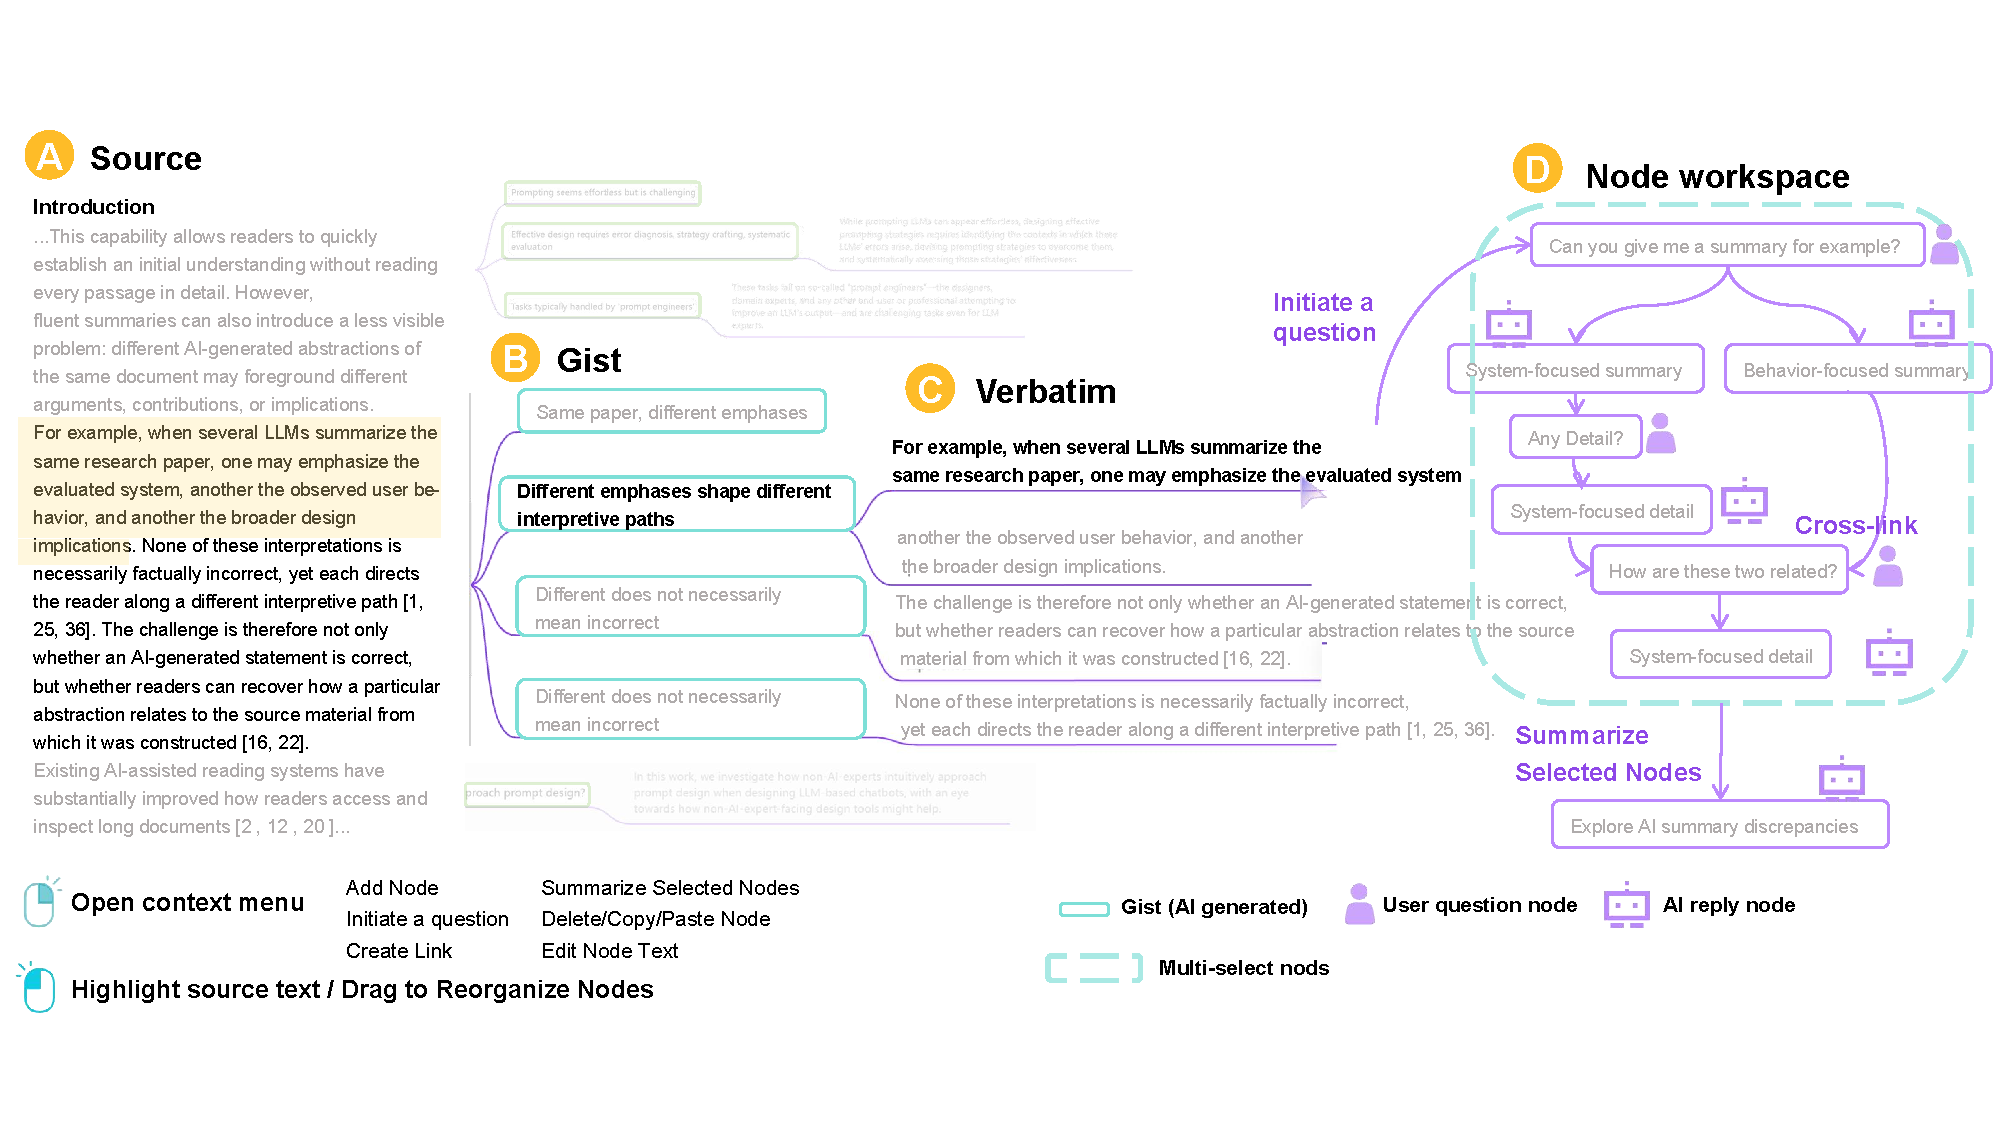
\includegraphics[trim=2 48 0 56, clip, width=\textwidth]{fig/gist_verbatim_foothold.pdf}
\caption{\textbf{StructWeaver overview.} Readers inspect the original source (A), navigate AI-generated gist units (B), and traverse their aligned verbatim evidence (C), with the corresponding source passage highlighted on selection. In the node workspace (D), readers can initiate follow-up questions, receive AI-generated responses grounded in the current interpretation path, create cross-links between nodes, and multi-select nodes to synthesize summaries across related interpretations. StructWeaver also supports node editing and reorganization through context-menu actions and drag-and-drop interactions.}
\label{fig:gist-verbatim-foothold}
\end{figure*}

\begin{figure*}[t]
\centering
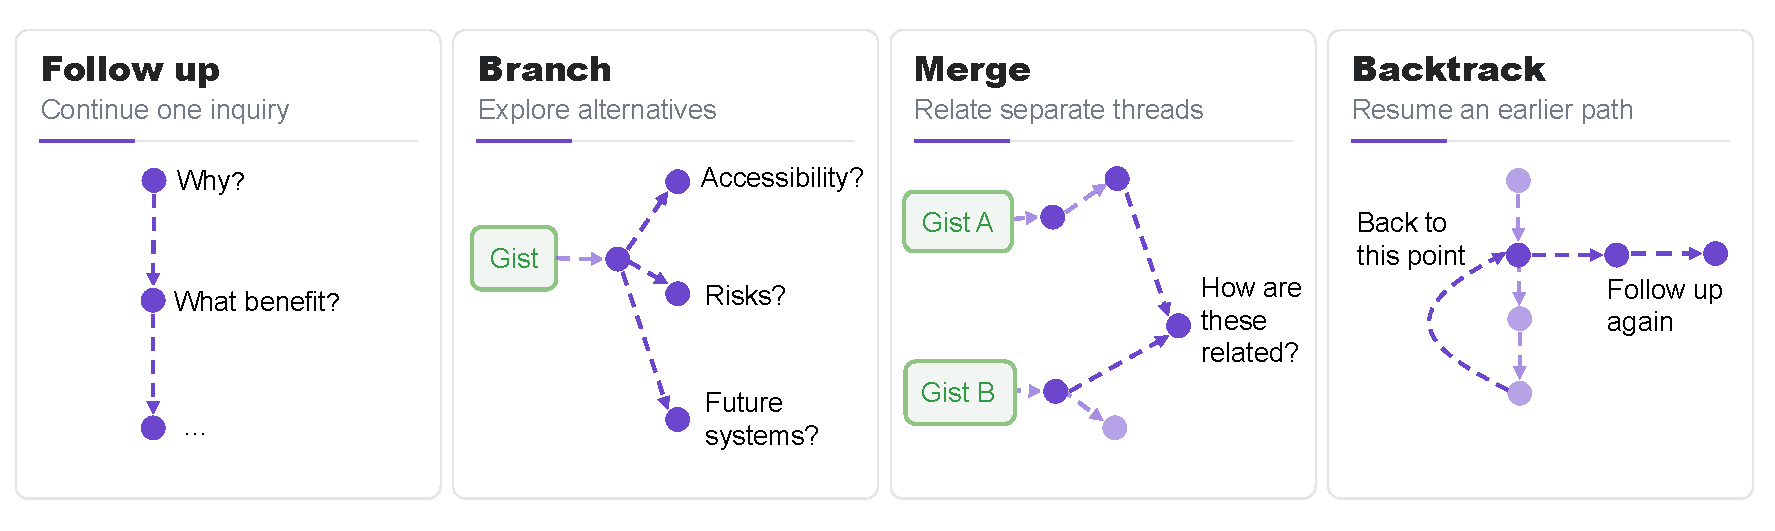
\includegraphics[width=\textwidth]{fig/concept_gvs_interaction.pdf}
\caption{\textbf{Recoverable interaction paths in StructWeaver.} The four examples show how readers continue one inquiry (\textit{Follow up}), explore alternatives (\textit{Branch}), relate separate threads (\textit{Merge}), and resume an earlier path (\textit{Backtrack}).}
\label{fig:concept-gvs}
\end{figure*}

\subsection{Structuring Gist into Revisitable Units}
\label{sec:interface}

To help readers establish stable interpretive anchors rather than relying on monolithic AI-generated summaries (DG1), StructWeaver represents AI-generated gist as a hierarchical node structure that follows the organization of the source document. This representation decomposes an overview into smaller units that readers can inspect, revisit, and extend independently while retaining their relationship to the document as a whole.

\subsubsection{Node Workspace}
The node workspace provides a tree-based representation of the reading process rather than a linear conversation history. StructWeaver draws on the visual diagramming tradition but constrains its initial representation to the document hierarchy, using the diagram as a navigational scaffold rather than requiring readers to author a free-form semantic graph. The initial tree follows the source document's heading hierarchy, preserving the organizational structure provided by the author. Within this structure, StructWeaver represents information using three types of nodes: \textit{document nodes} preserve section headings and document organization; \textit{gist nodes} contain AI-generated interpretations decomposed into sentence-level units; and \textit{verbatim nodes} retain source sentences associated with individual gist units. This organization allows readers to move across different levels of abstraction while maintaining where each interpretation originates in the document.

The workspace is vertically scrollable: readers can move down a branch by scrolling through the page rather than panning across a wide canvas. In practice, descending through document and gist nodes therefore feels closer to reading a linear gist sequence than to navigating a dense two-dimensional map, which helps keep deep trees readable even as more sections and follow-up branches are generated.

\subsubsection{Gist Nodes}
Instead of presenting a paragraph-level summary as a single completed response, StructWeaver decomposes each generated gist into smaller sentence-level units and places them beneath the corresponding document structure. Each gist node functions as an interpretive anchor that can be inspected or extended independently. For example, when a paragraph contains multiple claims or concepts, readers can focus on one gist unit without navigating through an entire generated response. This decomposition allows readers to progressively construct an understanding of the document while retaining the broader context in which each interpretation appears.

\subsubsection{Node-based Operations}
StructWeaver supports direct manipulation of the reading structure through node-level interactions. Readers can select individual nodes to inspect their corresponding content, expand or collapse branches to control the amount of visible information, and drag nodes to reorganize their workspace according to their evolving interpretation. Readers can also right-click a node to ask a follow-up question about the selected concept or evidence. Rather than creating an independent conversation, StructWeaver attaches the resulting question node to the selected branch, allowing subsequent exploration to remain associated with the interpretation that motivated it.

\subsection{Facilitating Gist--Verbatim Correspondence}
\label{sec:text-to-concept}

To reduce the effort required to reconstruct relationships between AI-generated interpretations and source passages (DG2), StructWeaver maintains explicit correspondence between gist nodes and verbatim evidence. This correspondence allows readers to traverse directly between an AI abstraction and the source text associated with it instead of manually searching across chat and document interfaces.

\subsubsection{Showing Corresponding Evidence}
Each gist unit is linked to one or more verbatim nodes representing sentences from the corresponding source paragraph (Figure~\ref{fig:gist-verbatim-foothold}). Readers can therefore descend from an AI-generated interpretation to the underlying source evidence within the same node structure. Selecting a verbatim node automatically navigates the verbatim panel to the corresponding location in the PDF and highlights the source passage. This interaction allows readers to inspect evidence without copying text, issuing an additional query, or manually locating the relevant passage in the document. In practice, the two source views play complementary roles: verbatim nodes support a brief glance at the specific wording that backs a gist unit, while the linear PDF helps readers confirm where they are in the author's progression and reduces the cost of orienting themselves solely through spatial node exploration. The correspondence also operates in the opposite direction. Because verbatim nodes remain embedded within the gist hierarchy, readers can return from a source passage to the interpretation through which it was encountered. StructWeaver therefore treats movement between gist and verbatim evidence as a continuous reading operation rather than a transition between two independent interfaces.

\subsubsection{Maintaining Source Structure}
StructWeaver preserves the author's original heading hierarchy when constructing Gist--Verbatim relations. Gist nodes are generated locally within paragraphs and remain attached to their corresponding document sections, preventing semantically similar content from different parts of the paper from being collapsed into a single global summary. This localized organization provides readers with both the AI's abstraction and the structural context in which the source material originally appears.

\subsection{Preserving Recoverable Interpretation Paths}
\label{sec:interpretation-paths}

To help readers recover previous lines of inquiry after switching between AI responses and source materials (DG3), StructWeaver organizes follow-up interactions around persistent branches rather than a global linear chat history. Each branch records how a reader moved from an initial interpretation to source evidence and subsequent questions, externalizing the trajectory of the reader's evolving understanding.

\subsubsection{Branch-based Questioning}
Readers can initiate a follow-up question from any document, gist, verbatim, or previously generated question node. StructWeaver attaches the new response to the selected node rather than appending it to the end of a global conversation. The detailed response is displayed in the AI response panel, while the corresponding node remains positioned within the interpretation path that produced it. For example, a reader examining one claim in a generated gist can inspect its supporting source passage, ask for clarification about that passage, and later return to the same branch without reconstructing the preceding conversational context.

\subsubsection{Path-based Context}
Follow-up questions are generated using the context associated with the selected path rather than the entire interaction history (Appendix~\ref{appendix:context}, Algorithm~\ref{alg:context}). StructWeaver constructs this context from relevant document structure, gist units, source evidence, and previous interactions along the active branch. This localized context reduces interference from unrelated questions and keeps model responses aligned with the interpretation currently being examined.

\subsubsection{Reorganizing and Recovering Reading Paths}
As readers develop different interpretations of a document, they can expand, collapse, and reorganize branches in the node workspace. Unlike a chronological chat history, where related exchanges may become separated by subsequent questions, the node structure preserves relationships according to what readers were investigating. StructWeaver thereby aligns three representations involved in AI-assisted reading---the AI's interpretation, the author's source structure, and the reader's evolving inquiry---within a persistent workspace that can be revisited and extended over time.

\subsection{System Implementation}
\label{sec:implementation}

StructWeaver implements the above interactions through a four-stage pipeline consisting of document preprocessing, localized gist generation, Gist--Verbatim alignment, and path-grounded response generation. The system maintains separate document, vector, and graph indexes to preserve the source structure, semantic representations, and relationships among nodes used during interaction.

\subsubsection{Document Processing and Gist Generation}
When a reader imports a PDF, StructWeaver first converts the document into a structured representation that preserves section headings, paragraphs, and individual source sentences. The resulting hierarchy is used to construct document nodes in the workspace. To prevent generated abstractions from losing their local source context, StructWeaver processes the document at the paragraph level rather than generating a single document-level summary.

For each paragraph, StructWeaver prompts DeepSeek-V4-Flash to generate a localized gist and subsequently decomposes the generated text into sentence-level gist units. These units become gist nodes associated with the original paragraph and heading hierarchy. This localized generation strategy allows the interface to present interpretable units at multiple levels of abstraction while retaining the location from which each abstraction was generated.

\subsubsection{Gist--Verbatim Alignment}
Using an LLM to independently extract supporting evidence would introduce another generative step between the reader and the source document. We therefore implement Gist--Verbatim correspondence using an embedding-based alignment procedure rather than asking the language model to select quotations.

For each paragraph, StructWeaver encodes every generated gist unit and source sentence into a shared embedding space and computes their pairwise cosine similarities. It then applies an order-preserving dynamic programming algorithm to assign each source sentence to exactly one gist unit while maximizing the total semantic similarity of the alignment (Appendix~\ref{sec:appendix-algorithms}, Algorithm~\ref{alg:alignment}; Figure~\ref{fig:dp-alignment}). Constraining alignment within individual paragraphs preserves local discourse structure and reduces matches between semantically similar sentences appearing in unrelated sections. The resulting assignments are represented as Gist--Verbatim edges in the node graph and used to support source highlighting and evidence traversal in the interface.

\begin{figure*}[t]
\centering
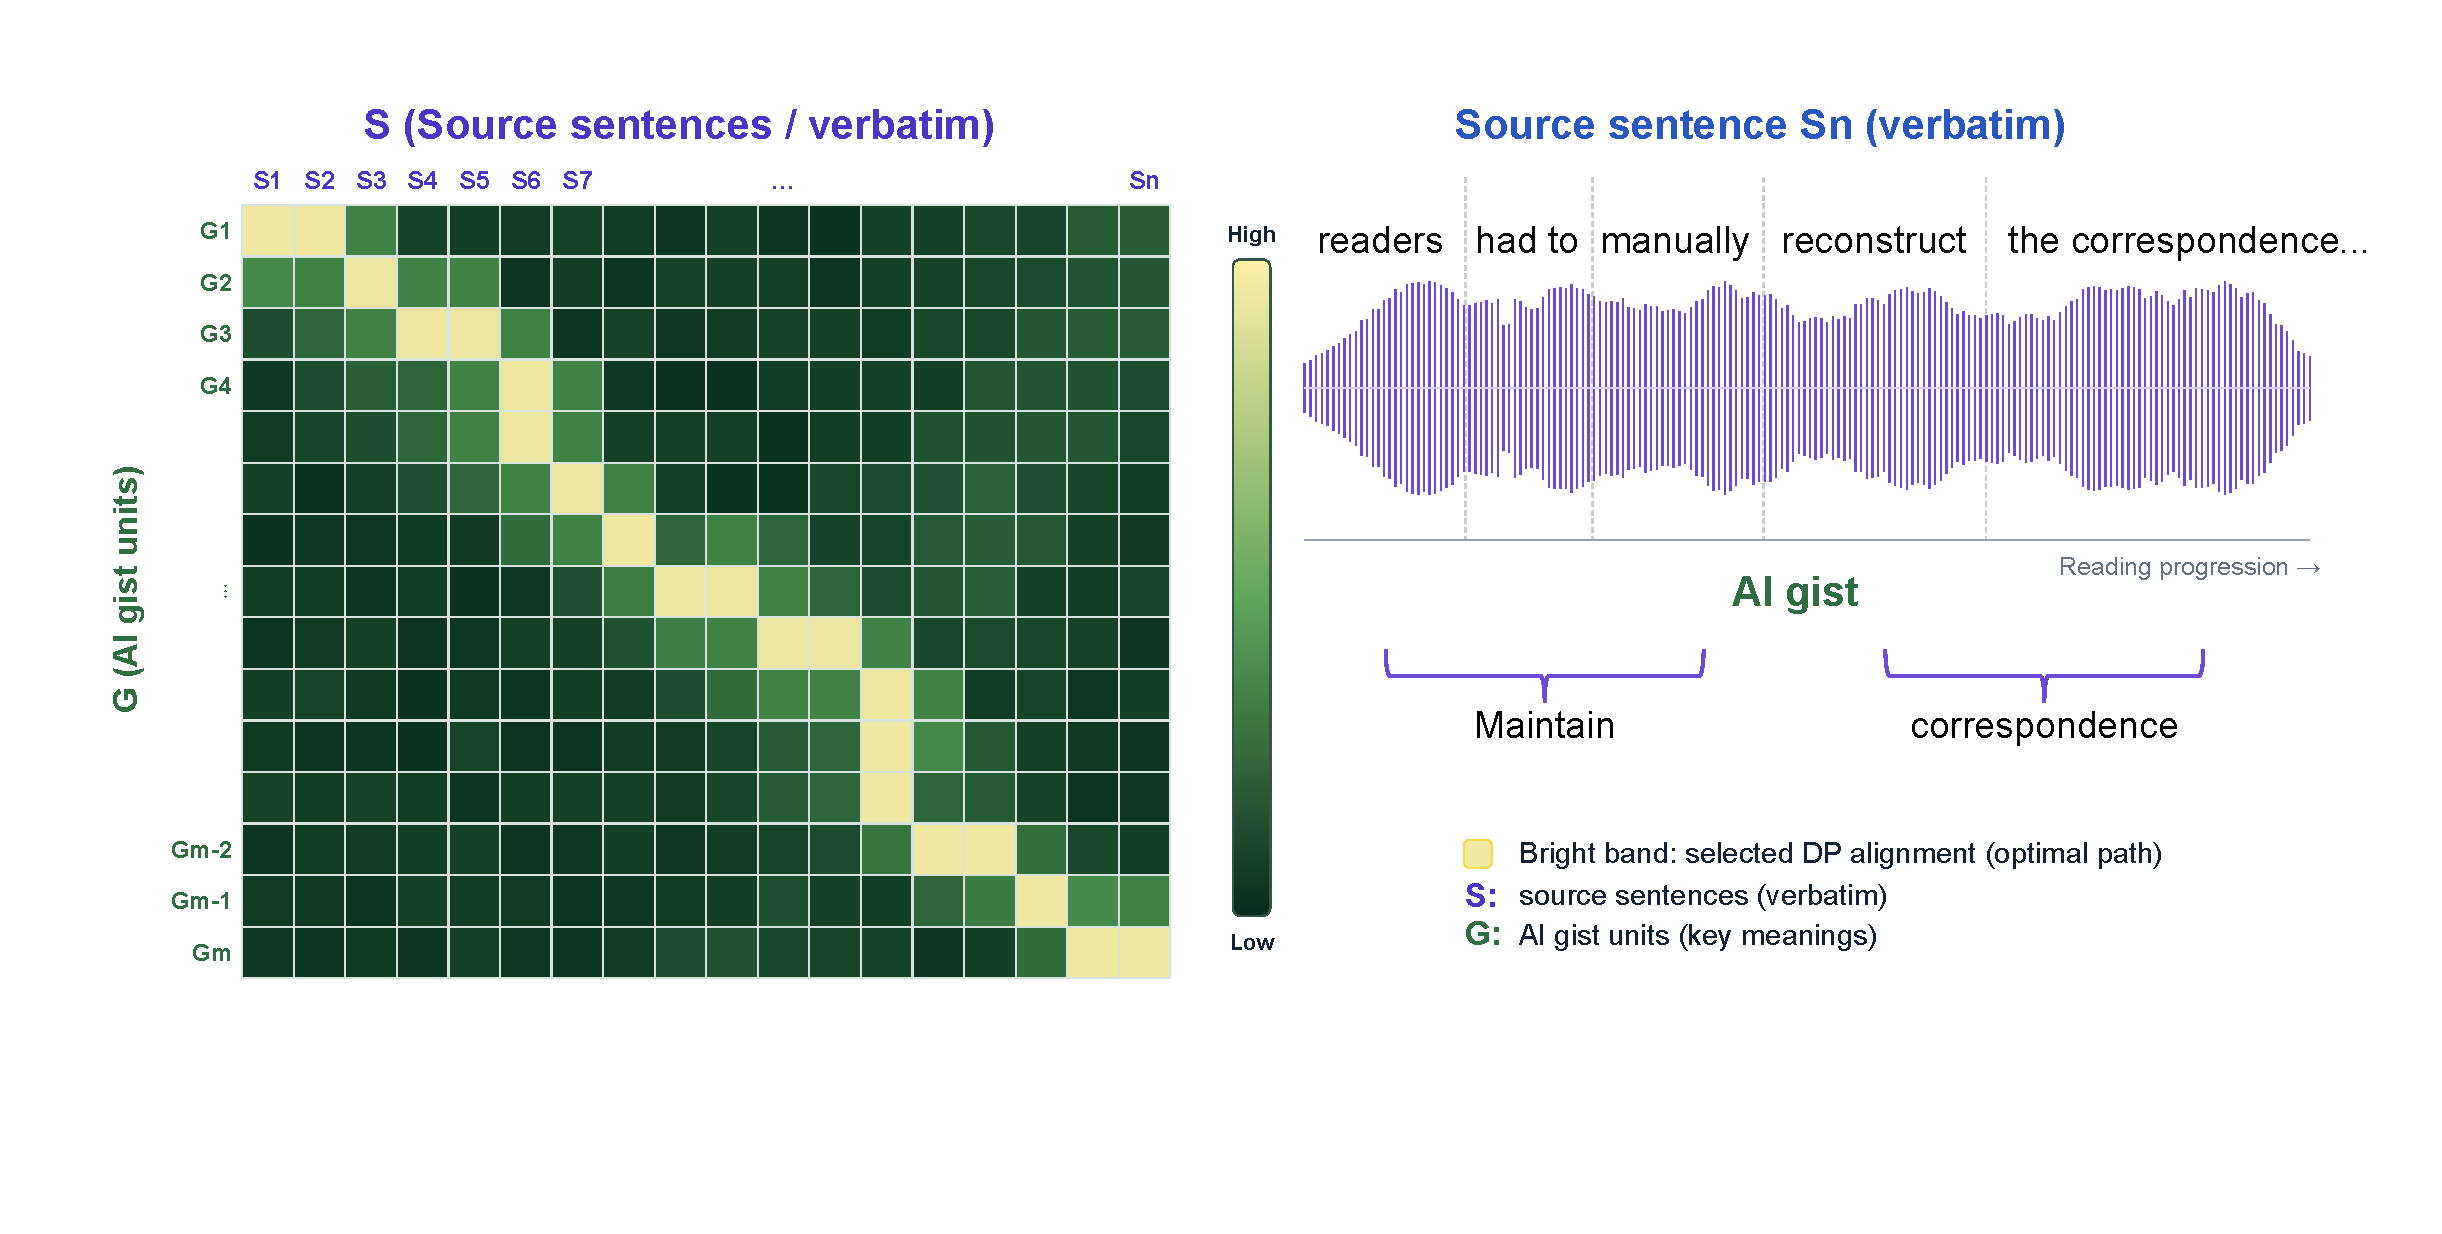
\includegraphics[trim=55 125 35 50, clip, width=\textwidth]{fig/algorithm_dp_alignment.pdf}
\caption{Semantic key-frame alignment between AI gist and source sentences. Inspired by sequence alignment in speech processing, StructWeaver treats gist units as compact semantic key frames over the source's semantic progression. It uses embedding-based cosine similarity and order-preserving dynamic programming to recover the maximum-similarity alignment, enabling each gist to serve as a direct entry point to its supporting verbatim evidence.}
\label{fig:dp-alignment}
\end{figure*}

\subsubsection{Path-grounded Question Answering}
When a reader asks a follow-up question from a node, StructWeaver constructs the model context from the selected branch rather than forwarding the complete interaction history. The context includes the relevant document section, gist units, aligned verbatim evidence, and preceding question--response pairs along the active path (Appendix~\ref{appendix:context}, Algorithm~\ref{alg:context}). The model-generated response is stored as a new node attached to that path and displayed in the AI response panel.

This path-based construction serves two purposes. First, it provides the model with the source and interpretive context most relevant to the reader's current question. Second, it prevents unrelated branches from progressively contaminating the prompt context as the reading session grows. Thus, the same graph structure used to externalize the reader's interpretation also determines the context used for subsequent AI interactions.

\subsubsection{Representation and Indexing}
StructWeaver persists three complementary representations of each reading session. The \textit{document index} maintains the hierarchical organization and locations of source passages; the \textit{vector index} stores semantic embeddings used for Gist--Verbatim alignment and retrieval; and the \textit{graph index} records parent--child relations among document, gist, verbatim, and question nodes. Together, these indexes allow the system to recover both where information appears in the source document and how it has been incorporated into the reader's evolving interpretation path.

\subsection{Representation Reliability Analysis}
\label{sec:reliability}

Because StructWeaver relies on automatically generated Gist--Verbatim correspondence to support evidence traversal, we further examined whether the resulting representation was sufficiently reliable for use as a reading scaffold. We generated alignments for 35 HCI papers, resulting in 3,054 AI-generated gist nodes, 11,881 evidence links, and 10,622 source sentences. Two authors independently inspected the generated relations and categorized each gist node as \textit{pass}, \textit{partial}, or \textit{fail}. Our goal was not to evaluate semantic alignment as an NLP benchmark, but to assess whether the generated relationships were sufficiently interpretable for readers to inspect the evidence underlying an AI-generated abstraction.

We identified four recurring sources of alignment error. First, \textit{rhetorical slot mismatches} occurred when semantically related goal, method, or conclusion statements were confused because the alignment procedure did not explicitly model discourse roles. Second, \textit{enumerated structure mismatches} occurred in passages containing similarly worded numbered items, such as ``Challenge 1/2/3'' or ``Contribution 1/2/3.'' Third, \textit{over-compressed gist units} occasionally combined several source claims into one abstraction, resulting in evidence that supported only part of the generated gist. Finally, \textit{document noise contamination} occurred when metadata, conference headers, DOI information, or citation fragments entered the candidate sentence pool. After excluding nodes affected primarily by PDF-to-Markdown parsing artifacts, two authors adjudicated 2,960 valid gist nodes. Table~\ref{tab:reliability} summarizes the resulting judgments.

\begin{table}[t]
\centering
\caption{Gist--Verbatim alignment reliability ($n=2{,}960$ valid gist nodes; 35 HCI papers).}
\label{tab:reliability}
\footnotesize
\setlength{\tabcolsep}{4pt}
\begin{tabularx}{\linewidth}{@{}l >{\raggedright\arraybackslash}X r@{}}
\toprule
Judgment & Criterion & Share \\
\midrule
Pass & Evidence fully supports gist & 61.9\% (1{,}831) \\
Partial & Same-paragraph direction; narrow coverage & 31.0\% (919) \\
Fail & Misalignment or unsupported linkage & 7.1\% (210) \\
\midrule
\multicolumn{2}{@{}l}{Acceptable (pass + partial)} & 92.9\% (2{,}750) \\
\bottomrule
\end{tabularx}
\end{table}

Overall, 92.9\% of valid gist nodes retained evidence that either fully supported the generated abstraction or remained within the same semantic direction with narrower coverage. These results informed our decision to expose Gist--Verbatim relations directly to readers rather than treating them as hidden system predictions. StructWeaver therefore presents each alignment as an inspectable correspondence between abstraction and source evidence: readers can immediately examine the linked passage, identify partial or incorrect support, and continue interpretation from the original text.







% \section{Evaluation}
% \label{sec:user-study}

% Because author, AI, and reader perspectives on a text admit no single ground truth, we evaluated StructWeaver as a behavioral intervention rather than a performance optimization system. Specifically, we asked: when AI-generated abstractions become traversable, how do readers coordinate AI interpretations, source evidence, and their own evolving understanding throughout reading?

% We address two research questions:

% \begin{itemize}[leftmargin=*, noitemsep]
% \item RQ1: How does traversable AI reading change readers' reading processes?
% \item RQ2: How do these process changes affect reading outcomes and subjective experiences?
% \end{itemize}

% \subsection{Study Design}

% We conducted a paired within-subject study comparing StructWeaver against a baseline AI-assisted reading workflow consisting of a conventional chat interface alongside a PDF viewer.

% Twelve participants (P01--P12), distinct from the formative study participants (T01--T12), completed reading tasks under both conditions. Condition order was counterbalanced.

% Participants were asked to read unfamiliar research papers and prepare a written summary describing their understanding of each paper. We intentionally selected unfamiliar topics to encourage reliance on both AI interpretations and source materials rather than prior expertise.

% Each session consisted of four phases:
% \begin{enumerate}[leftmargin=*, noitemsep]
% \item System tutorial;
% \item AI-assisted reading;
% \item Summary writing;
% \item Post-task questionnaires and semi-structured interviews.
% \end{enumerate}

% We collected screen recordings, written summaries, questionnaires, and interview responses throughout the study.

% \subsection{Measures}

% We evaluated three complementary dimensions.

% \paragraph{Reading Processes (RQ1).}
% We manually coded screen recordings to characterize how participants coordinated AI interpretations and source evidence during reading.

% \paragraph{Reading Outcomes (RQ2).}
% We evaluated written summaries as a descriptive quality guardrail (see \S\ref{sec:summary-eval}).

% \paragraph{Subjective Experiences (RQ2).}
% Participants completed post-task questionnaires examining cognitive burden, source awareness, structural understanding, and future adoption intentions, followed by semi-structured interviews.

% \subsection{Summary Evaluation}
% \label{sec:summary-eval}

% To construct reference targets, two authors first independently extracted key triples from each source paper. Each triple captured a core relation expressed in the paper, such as an argument, finding, cause--effect relation, or contribution. We then used the intersection of the two authors' extracted triples as the set of core points for each paper.

% We next segmented participants' written summaries into summary units and converted each unit into one or more triples. Two authors then evaluated these participant triples along two dimensions: whether the triple corresponded to one of the core reference triples, and whether it introduced unsupported or inaccurate information. Based on these annotations, we computed Recall, Precision, and Hallucination:
% \begin{itemize}[leftmargin=*, noitemsep]
% \item Recall = covered core triples / total core triples;
% \item Precision = accurate participant triples / all participant triples;
% \item Hallucination = unsupported or inaccurate participant triples / all participant triples.
% \end{itemize}

% Because these measures depend on unit segmentation and interpretive judgment, we treat them as descriptive quality checks for examining whether the workflow shift under StructWeaver introduced obvious quality costs.



\section{Evaluation Study}
\label{sec:evaluation}
\label{sec:user-study}

We conducted a within-subjects study to investigate how StructWeaver changes AI-assisted reading compared with a conventional chat-and-PDF workflow. Because StructWeaver is designed primarily to change how readers coordinate AI-generated abstractions with source evidence, we focused on observable reading processes and used subjective experience and summary quality to examine the consequences of these behavioral changes. Specifically, we asked: \textbf{RQ1:} How does StructWeaver affect how readers coordinate AI-generated gist and source evidence during reading? \textbf{RQ2:} How do these changes affect readers' reading outcomes and subjective experiences?

\subsection{Participants}

To validate the reading challenges identified in the formative study and to examine the effectiveness of StructWeaver, we recruited a new group of 12 participants (P01--P12; 7 male, 5 female; $M_{\mathrm{age}}=21.62$, $SD=3.15$), distinct from the formative interviewees (T01--T12). All participants were currently enrolled students who routinely needed to read academic literature. Their educational backgrounds included seven bachelor's students, four master's students, and one doctoral student. Disciplines spanned computer science ($n=6$) as well as mathematics, biomedicine, materials science, biological science, basic medicine, and automation engineering. Eligibility required regular experience with AI dialogue systems (e.g., chatbots or AI-assisted tools) and with long-form reading such as academic papers or textbooks; diversity in the sample therefore came primarily from educational stage and disciplinary background rather than from mixing novice and expert AI users.

\subsection{Study Design}

We compared the StructWeaver condition with the Baseline condition, which consisted of ChatGPT alongside a PDF viewer (Figure~\ref{fig:study-interfaces}, left). Participants completed AI-assisted reading tasks on two unfamiliar HCI research papers---\textit{Why Johnny Can't Prompt}~\cite{Zamfirescu-Pereira} and \textit{Synthetic Lies}~\cite{synthetic_lies}---and subsequently wrote a summary describing their understanding of each paper. We selected these papers because they are long-form CHI contributions outside most participants' primary research niches, reducing reliance on prior domain knowledge and encouraging coordination between AI-generated interpretations and the source text. Paper--condition assignment was counterbalanced together with interface order. Before the main tasks, eligibility for AI-assisted long-text reading was checked using a pool of additional HCI papers on dialogue agents, sensemaking, scholarly synthesis, and related topics (Appendix~\ref{appendix:study-materials}). Participants worked at their own pace; reading a paper typically took on the order of 15--35 minutes before writing the summary. Appendix~\ref{appendix:walkthrough} reconstructs an illustrative participant session from screen recordings and debrief.

\begin{figure*}[t]
\centering
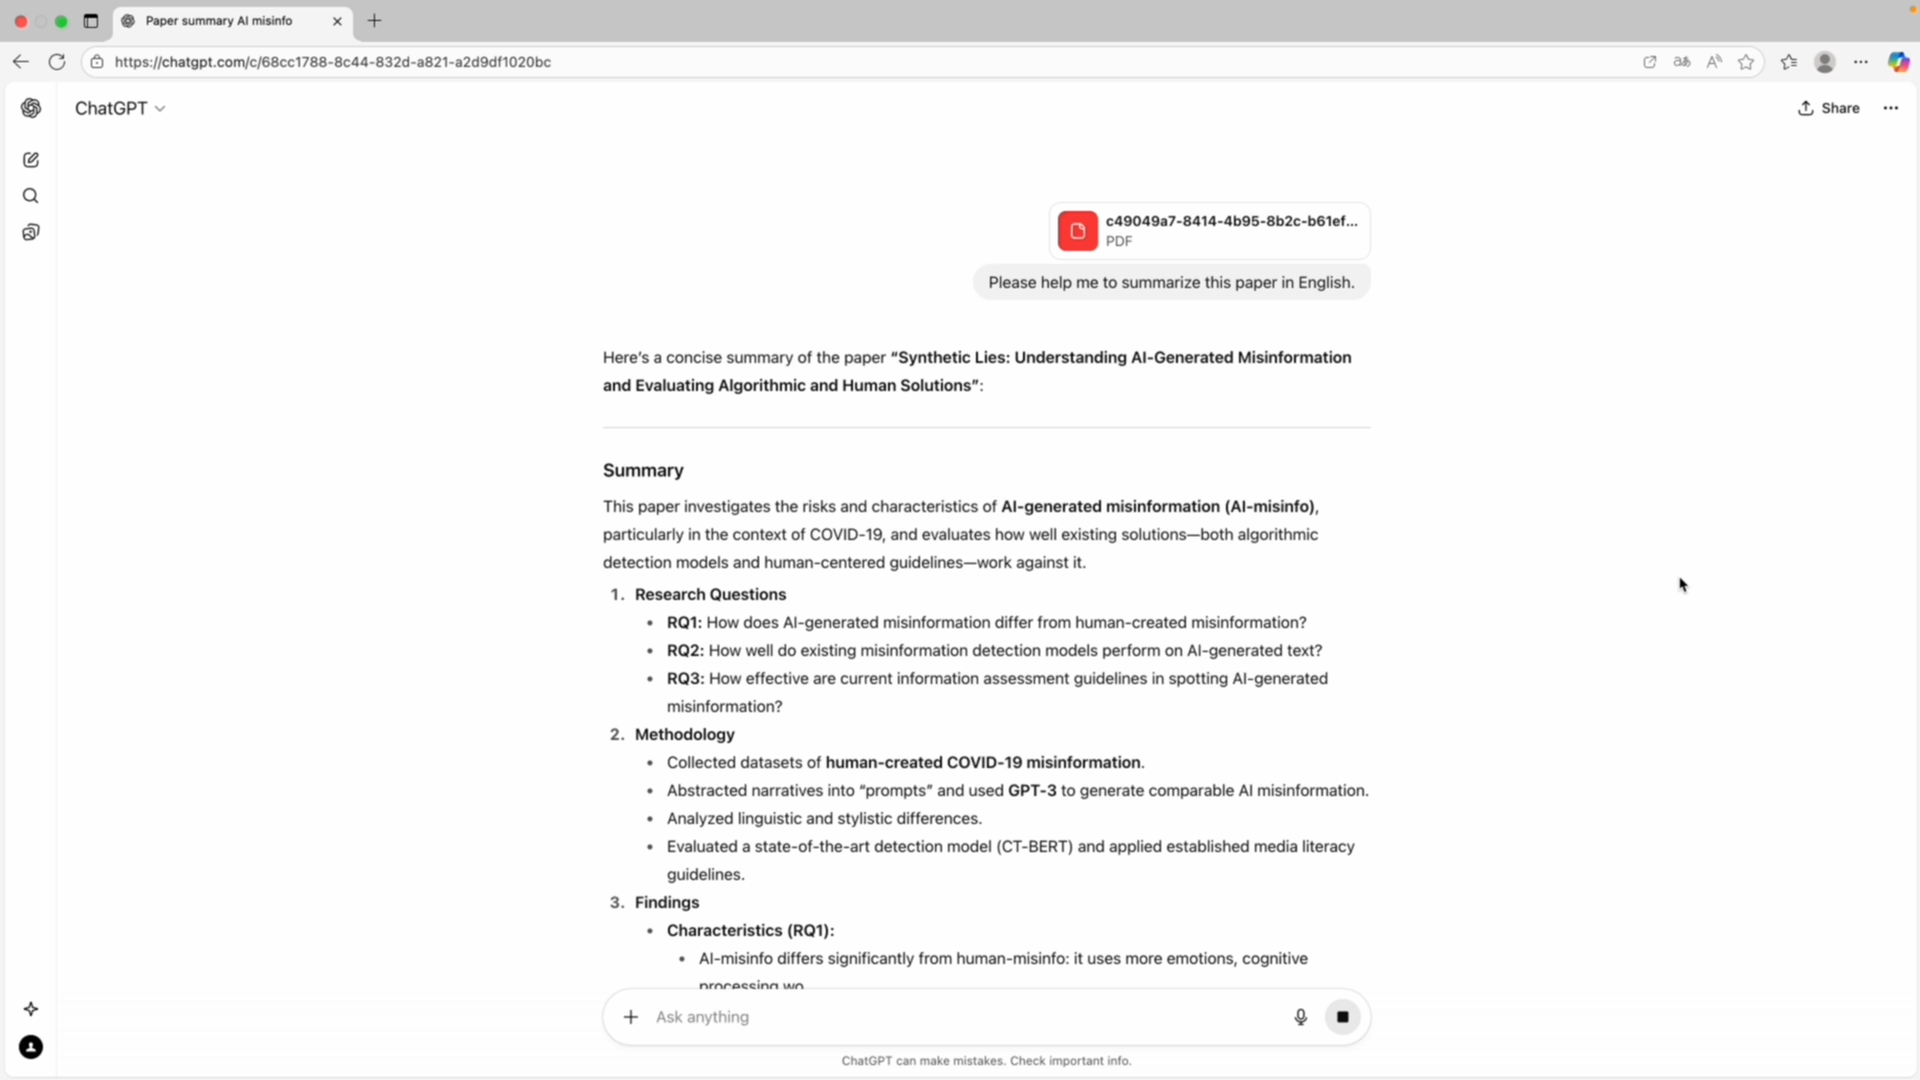
\includegraphics[width=0.44\textwidth]{fig/baseline.png}
\hfill
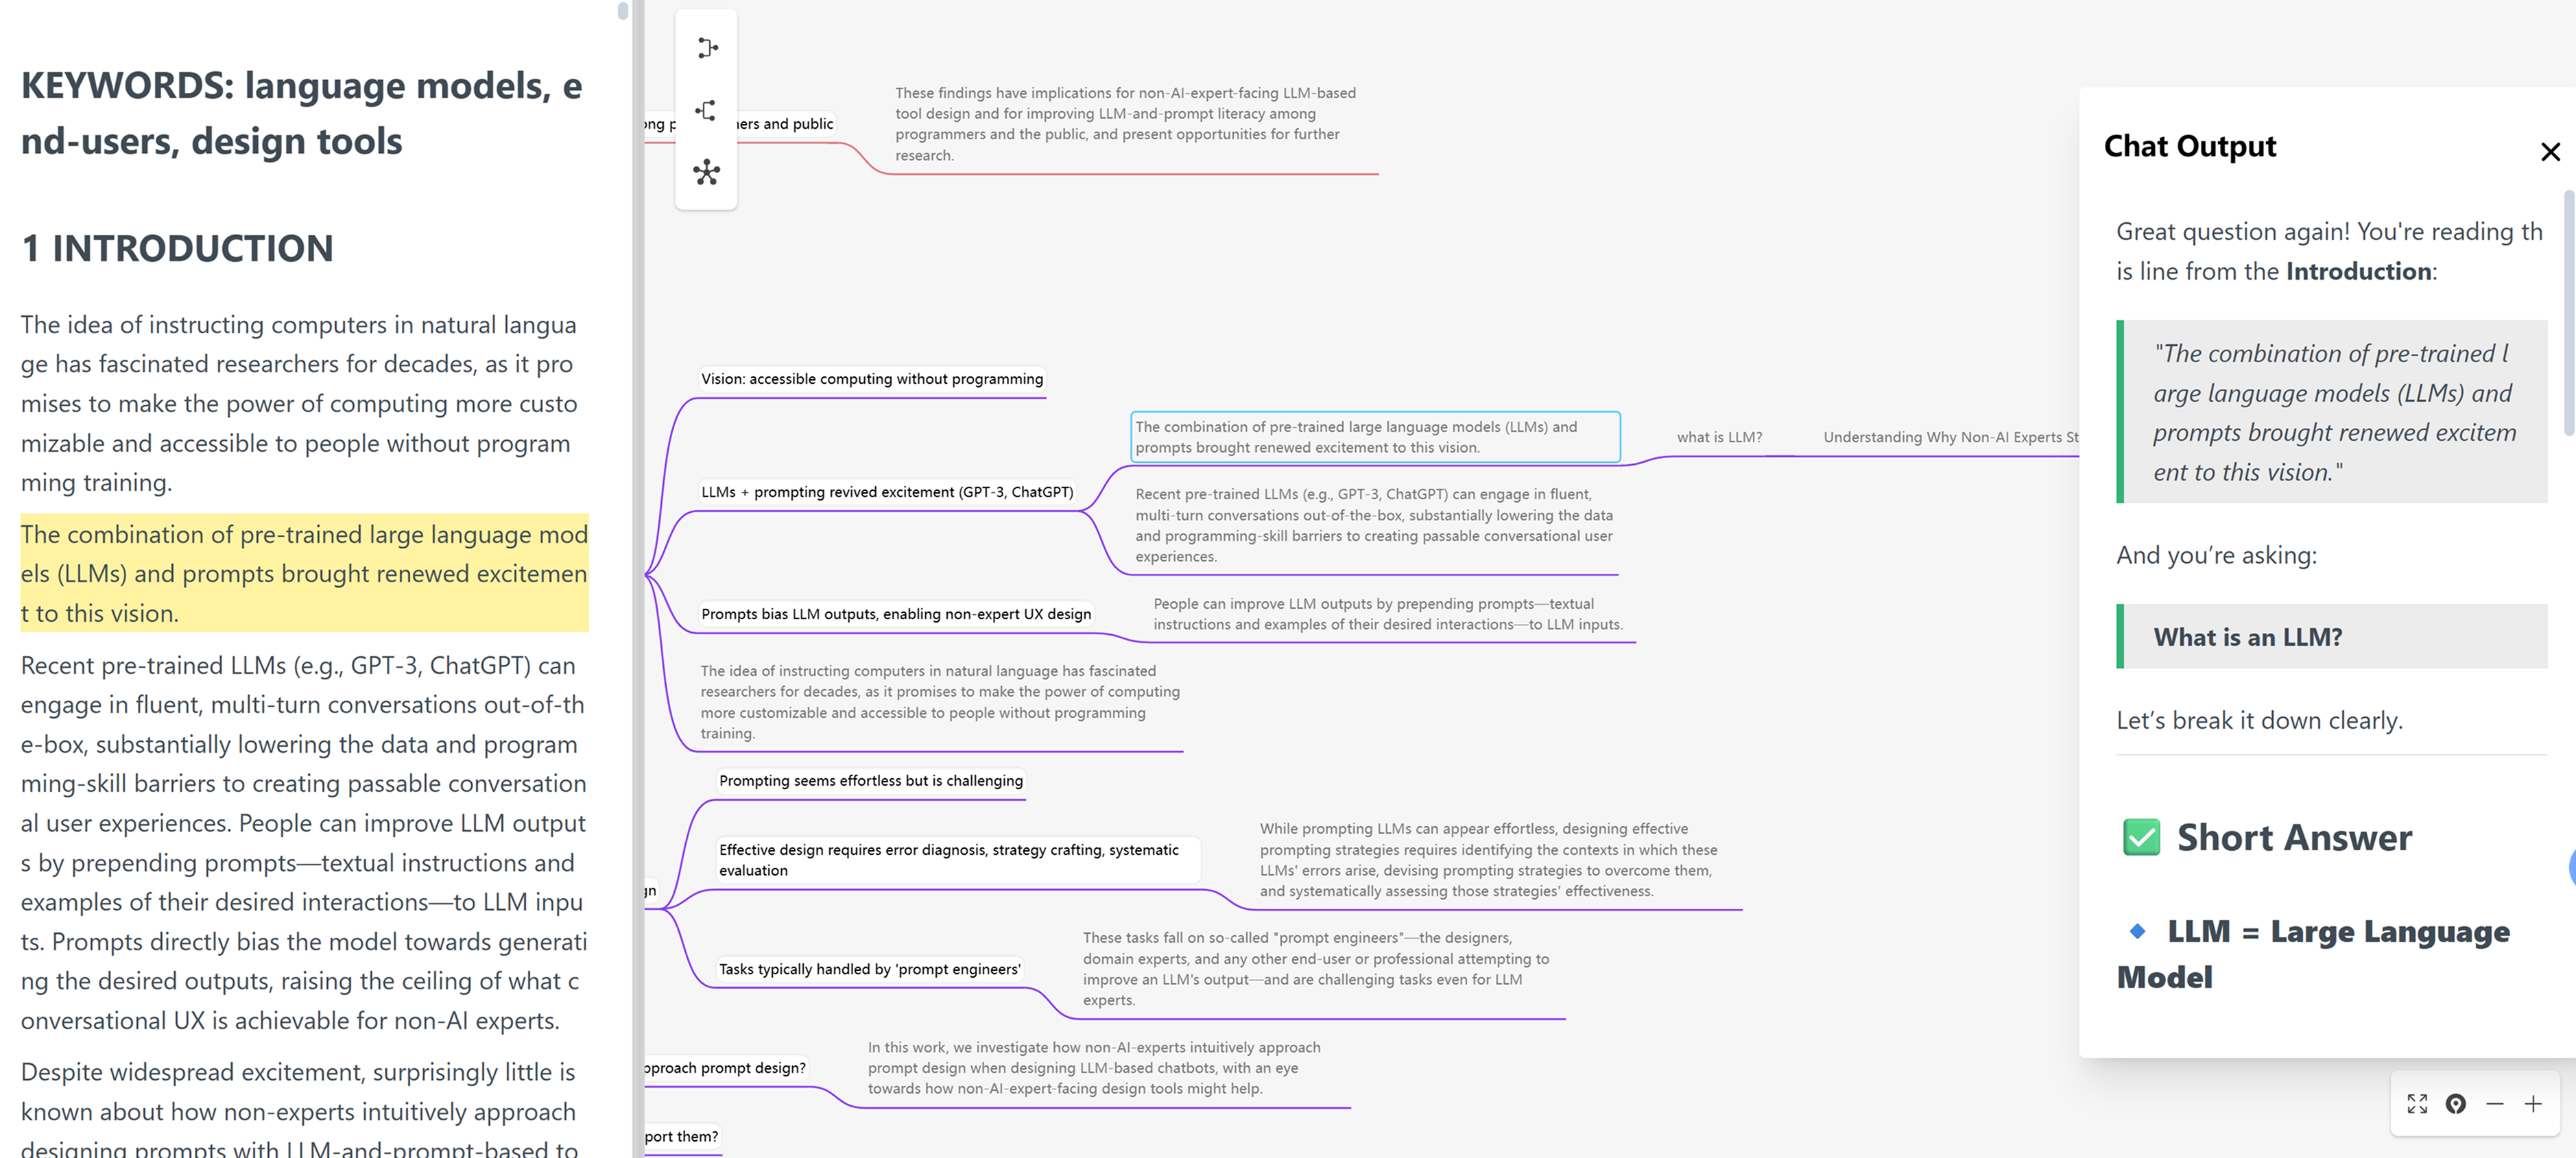
\includegraphics[width=0.52\textwidth]{fig/system.png}
\caption{Study interfaces shown to participants. \textbf{Left (Baseline):} ChatGPT alongside a PDF viewer; AI responses and source text remain in separate panes. \textbf{Right (StructWeaver):} hierarchical node workspace with gist--verbatim alignment, verbatim panel, and AI response panel.}
\label{fig:study-interfaces}
\end{figure*}

Each participant completed one reading task in the StructWeaver condition and one in the Baseline condition, with condition order counterbalanced across participants. Before using each interface, participants received a tutorial introducing its primary interactions. During each task, participants read the assigned paper with AI assistance and determined how to allocate their attention between AI-generated content and the source document. They then wrote a summary based on their understanding of the paper, completed a post-task questionnaire, and participated in a semi-structured interview reflecting on their reading process and experience. We collected screen recordings, written summaries, questionnaire responses, and post-task interview data for subsequent analysis.

\subsection{Measures and Analysis}

We evaluated StructWeaver along three complementary dimensions: reading behavior, subjective experience, and summary quality.

\paragraph{Reading Behavior.}
To examine how participants coordinated AI-generated interpretations and source evidence (RQ1), we drew on established procedures for coding and quantifying recorded qualitative data~\cite{chi1997quantifying}. Three authors watched the screen recordings and coded observable reading actions along each session timeline (Figures~\ref{fig:behavior-timeline} and~\ref{fig:behavior-binned}). Disagreements were resolved through discussion until consensus. The scheme used six mutually exclusive categories aligned with the figure legends:
\begin{itemize}[leftmargin=*, noitemsep]
    \item \textbf{Summarization}: requesting a full-document, sectional, or otherwise compressed overview of the paper, or asking the model to shorten or restructure a prior summary;
    \item \textbf{Understanding}: asking for explanations of concepts, terms, nodes, methods, or argumentative points without primarily seeking compression;
    \item \textbf{Examples \& Relations}: requesting examples, comparisons, or associations that connect claims, RQs, or parts of the paper;
    \item \textbf{Chat Management}: returning to prior chat turns, reusing earlier answers, or correcting/clarifying a previous exchange (including reviewing chat history);
    \item \textbf{Source Reading}: viewing or scrolling the linear PDF as independent reading, not as an immediate follow-through from an AI/node evidence jump;
    \item \textbf{Source Grounding}: reconnecting an AI-generated interpretation with source evidence---e.g., jumping from a gist node to its linked passage, asking the model for supporting/alignment text, or reading the cited snippet immediately after such a jump.
\end{itemize}
We compared within-participant category frequencies between conditions using Wilcoxon signed-rank tests with Holm correction across the six categories. We further examined the recordings together with post-task interviews to characterize how participants used Gist--Verbatim traversal during interpretation.

\paragraph{Subjective Experience.}
To examine participants' perceived experience under the two workflows (RQ2), we administered a study-specific 11-item post-task questionnaire using 7-point Likert scales. Its design was informed by a differentiated cognitive-load instrument covering intrinsic, extraneous, and germane load~\cite{leppink2013development} and by a global mental-effort item~\cite{paas1992training}; we adapted the wording and response scale to AI-assisted long-text reading. The questionnaire examined cognitive load associated with understanding document logic, maintaining and integrating information, controlling information granularity, organizing document structure, reading with explicit concepts or questions, and overall task effort. Across all 11 study-specific items, Cronbach's $\alpha$ was $.82$. Because responses were paired and ordinal, we compared the StructWeaver and Baseline conditions using Wilcoxon signed-rank tests. Post-task interviews were used to contextualize questionnaire responses and identify why particular interactions increased or reduced perceived effort.

\paragraph{Summary Quality.}
To examine whether changes in reading behavior introduced evident costs to participants' resulting understanding (RQ2), we evaluated their written summaries using reference-based measures of content coverage and factual accuracy. We treated these measures as descriptive quality checks rather than the primary performance objective of StructWeaver, as described below.

\subsection{Summary Evaluation}
\label{sec:summary-eval}

Drawing on semantic content-unit and relation-based approaches to summary evaluation~\cite{nenkova-passonneau-2004-evaluating,hovy-etal-2006-automated}, we developed a study-specific, structure-aware analysis. All reported summary-quality scores follow this relational-triple procedure; the two annotators were paper authors rather than external domain experts (analysis worksheets sometimes labeled the same author pass as ``expert'' scoring).

To construct reference targets for each paper, the two authors independently extracted relational triples representing core claims in the source introductions (29 cores for \textit{Synthetic Lies}~\cite{synthetic_lies}; 22 for \textit{Why Johnny Can't Prompt}~\cite{Zamfirescu-Pereira}). Each triple encoded a subject, relation, and object for a claim central to the paper (e.g., an argument, finding, causal relationship, or contribution). We retained triples independently identified by both authors as the core reference set.

We then segmented each participant's written summary into semantic units and represented each unit as one or more relational triples. The same two authors evaluated participant triples along two dimensions---(1)~whether a triple corresponded to a core reference relation and (2)~whether it contained information unsupported by or inconsistent with the source~\cite{maynez-etal-2020-faithfulness}---with units from both conditions interleaved and scored without condition labels visible (blind unit review). Units too vague to credit were excluded from precision and hallucination denominators. Based on these annotations, we computed three descriptive measures per summary:
\begin{itemize}[leftmargin=*, noitemsep]
    \item \textbf{Recall}: distinct core reference triples covered / number of cores for that paper;
    \item \textbf{Precision}: accurate participant triples / non-vague participant triples;
    \item \textbf{Hallucination}: inaccurate participant triples / non-vague participant triples.
\end{itemize}

We analyze these scores at two complementary grains. At the \emph{participant} level, we compare paired condition means with Wilcoxon signed-rank tests ($n=12$). At the \emph{pooled-triple} level, we additionally report $\chi^2$ tests on contingency tables that pool accurate vs.\ inaccurate triples (and covered vs.\ uncovered cores) across participants; these tests describe pooled counts and do not treat nested triples as independent observations. Because constructing reference triples, segmenting summaries, and judging correspondence involve interpretive decisions, we use the measures primarily as a quality guardrail rather than as a standalone reading-performance score.

\subsubsection{Annotation Reliability}

Agreement was higher for individual relational triples than for whole-summary judgments. For hallucination judgments at the triple level, the two author-annotators achieved 92.6\% raw agreement with Cohen's chance-corrected agreement coefficient~\cite{cohen1960coefficient} ($\kappa=.535$). Agreement on whether participant triples corresponded to core reference points was likewise $\kappa\approx.60$, depending on the annotation criterion. We also observed a systematic difference in annotation tendencies, with one author making significantly more hallucination judgments than the other (McNemar $\chi^2=6.67$, $p=.010$). At the summary level, agreement was substantially lower: when annotators judged whether an entire participant summary should be considered hallucinatory, raw agreement decreased to 54.2\% ($\kappa=.083$). We therefore report Table~\ref{tab:summary_quality} and the associated tests from the author triple coding, treat whole-summary labels cautiously, and interpret pooled-triple $\chi^2$ in light of annotator-strictness differences.





% \section{Findings}
% \subsection{Behavioral Logs Show a Shift from Summary Consumption to Source Grounding}
% \label{sec:behavior-logs}

% Two authors first independently examined screen recordings and coded participants' observable reading actions; disagreements were resolved through discussion. The coding scheme included summarization/compression, understanding/explanation, source reading, source grounding, example/association, and conversation management. Source grounding refers to actions that explicitly reconnect AI interpretations with source evidence, such as jumping from a gist node to the original passage, comparing AI-generated nodes with source sentences, or clicking links provided in AI chat responses.

% \begin{figure*}[t]
% \centering
% \includegraphics[width=\textwidth]{fig/compact_behavior_combined.png}
% \caption{Behavioral shift from summary consumption to source grounding ($n=12$). Left: per-participant change in coded action counts (StructWeaver $-$ Baseline). Right: group-level proportions by condition. Summarization/compression decreased while source grounding increased under StructWeaver (Wilcoxon signed-rank tests; Holm-corrected).}
% \label{fig:behavior-shift}
% \end{figure*}

% The behavioral logs revealed a clear shift in the dominant form of AI-assisted reading (Figure~\ref{fig:behavior-shift}). In the baseline condition, participants' interactions were largely organized around summarization and compression: they asked AI to condense the paper, reformulate sections, or provide a compact overview. By contrast, under StructWeaver, participants' interactions were dominated by source grounding. Rather than treating AI outputs as terminal responses, participants repeatedly moved between AI-generated gist and source evidence.

% This shift suggests that StructWeaver reconfigured AI-assisted reading from summary consumption toward source-grounded understanding construction. Importantly, verification did not appear only as a separate activity triggered by explicit doubt. Instead, it became embedded in the ordinary movement between gist nodes and source passages.

% \subsection{Readers Used Gist--Verbatim Alignment for Interpretation Work}

% The behavioral logs show that StructWeaver shifted participants toward source grounding. To understand what this grounding was used for, we examined screen recordings and post-study interviews. We found that participants did not merely click evidence links to check isolated claims. Instead, they used Gist--Verbatim alignment for three forms of interpretation work.

% \paragraph{Interpretation inspection.}
% Participants used this alignment to inspect how AI organized the paper. By moving between gist nodes and linked source evidence, they could see which parts of the original text were being compressed into a particular interpretation. P11 described this as being able to know whether ``these summarized keywords or claims are actually supported by real information in the original text,'' and added that linking back to the source gave them more confidence in the mind map's claims.

% \paragraph{Omission detection.}
% Participants also used missing or weak source connections as cues that an AI abstraction might be incomplete. P03 noted that when many AI-generated points could be found in the original text, they seemed reliable, but unsupported points served as reminders to verify: ``there is also another category without source support; its role is to remind the user to verify.'' This shifted verification from asking only whether a statement was true toward asking what the AI interpretation might have failed to cover.

% \paragraph{Misalignment repair.}
% Participants further used source traversal to repair mismatches between AI interpretations and author arguments. P11 contrasted baseline AI, where the model ``comes with its own logic'' that the reader could only passively accept, with StructWeaver, where the structure was clearer, linked to the original text, and easier to modify. P03 similarly described using the system as a reference and then returning to the paper to judge for themselves.

% Taken together, these practices suggest that StructWeaver's alignment is not merely a citation mechanism. It does not explain the model's internal reasoning, but it makes the model's interpretive output inspectable: readers can examine how source evidence is compressed, where support is missing, and where the AI's interpretation may need repair.

% \subsection{Participants Experienced Verification as Easier to Perform}

% Questionnaire and interview responses further suggest that StructWeaver changed how verification felt to participants. The system did not simply make participants more skeptical of AI. Instead, it made verification easier to perform by keeping AI interpretations and source evidence on the same recoverable path.

% After each reading task, participants completed an 11-item cognitive load questionnaire (7-point Likert; Cronbach's $\alpha = .82$) comparing StructWeaver and baseline on intrinsic, extraneous, and germane load. Wilcoxon signed-rank tests ($n=12$) showed that StructWeaver reduced intrinsic load ($M=2.50$ vs.\ $3.69$, $\Delta=-1.19$, $p=.026$, $d=-0.74$) and extraneous load ($M=2.50$ vs.\ $3.44$, $\Delta=-0.94$, $p=.011$, $d=-0.87$), while increasing germane load ($M=5.20$ vs.\ $3.72$, $\Delta=+1.48$, $p<.001$, $d=1.85$). At the item level, significant improvements favored StructWeaver on Q1 (understanding logic/causality, $p=.016$), Q6 (adjusting content granularity, $p=.027$), Q8 (organizing structure/summarizing, $p=.049$), Q9 (reading with concepts/questions, $p=.002$), Q10 (integrating scattered information, $p=.006$), and Q11 (overall effort, $p=.008$); Q3 showed a marginal trend ($p=.059$), while Q2, Q4, Q5, and Q7 did not reach significance (Table~\ref{tab:survey_stats}).

% \begin{table}[t]
% \centering
% \caption{Wilcoxon signed-rank tests for cognitive load questionnaire items ($n=12$). Items 1--6 and 11 are negatively framed (lower is better under StructWeaver); items 7--10 are positively framed.}
% \label{tab:survey_stats}
% \small
% \begin{tabularx}{\linewidth}{c X c c}
% \toprule
% Q & Dimension & $p$ & Sig. \\
% \midrule
% 1 & Difficulty understanding logic/causality & .016 & * \\
% 6 & Need to adjust content granularity & .027 & * \\
% 8 & Proactively organizing structure/summarizing & .049 & * \\
% 9 & Reading with concepts/questions in mind & .002 & ** \\
% 10 & Integrating scattered information & .006 & ** \\
% 11 & Overall task effort & .008 & ** \\
% \midrule
% 3 & Difficulty maintaining/processing information & .059 & $\dagger$ \\
% \multicolumn{4}{l}{\textit{Non-significant: Q2, Q4, Q5, Q7}} \\
% \bottomrule
% \end{tabularx}
% \\[4pt]
% \footnotesize{$^{*}\,p<.05$, $^{**}\,p<.01$, $\dagger$ marginal ($p<.06$).}
% \end{table}

% Participants often described baseline AI reading as requiring them to mentally coordinate disconnected materials: a chat response, a PDF, and their own emerging understanding. Under StructWeaver, linked gist nodes reduced this reconstruction burden. P11 explained that baseline AI made it difficult to compare outputs with the original text, whereas StructWeaver allowed them to ``jump to the source with a click,'' making them more willing to compare whether evidence supported a claim.

% This distinction is important. The result is not simply that users trusted AI more or less. Rather, StructWeaver changed the conditions under which verification could happen. By making abstraction--evidence relations persistent and traversable, the system turned verification from an attitude-dependent decision into a capacity-supported reading action.


\section{Findings}
\label{sec:findings}

We present findings from behavioral logs, screen recordings, questionnaires, written summaries, and post-task interviews corresponding to our two research questions. Overall, StructWeaver changed both where participants directed their attention during AI-assisted reading and how they coordinated AI-generated interpretations with source evidence. Compared with the Baseline condition, participants engaged less in repeated summary compression and more frequently returned to the source. They used Gist--Verbatim traversal not only to verify individual claims, but also to inspect how AI compressed the paper, identify potentially incomplete interpretations, and resolve mismatches between AI-generated structure and the author's argument. Questionnaire results further suggest that these behavioral changes reduced the effort required to coordinate disconnected representations while increasing participants' engagement in organizing and integrating the material. At the participant level, summary quality (Recall, Precision, and Hallucination) showed no stable significant system advantage; pooled-triple $\chi^2$ associations were annotator-sensitive, so we treat them as descriptive rather than as a robust outcome claim.

\subsection{From Summary Consumption to Source Grounding}
\label{sec:behavior-logs}

Behavioral logs showed a clear difference in how participants interacted with AI across the two conditions (Figures~\ref{fig:behavior-timeline} and~\ref{fig:behavior-binned}). In the Baseline condition, participants' interactions were largely organized around summarization and compression: they repeatedly asked AI to condense the paper, reformulate sections, or provide compact overviews. In the StructWeaver condition, summarization/compression actions decreased while source-grounding actions increased. Rather than treating AI-generated responses as terminal outputs, participants more frequently traversed between generated gist and corresponding passages in the source document. Wilcoxon signed-rank tests on per-participant category counts ($n=12$; Holm-corrected across six categories; Table~\ref{tab:behavior_stats}) showed significant increases in Source Grounding ($M=6.00$ vs.\ $0.25$; $\Delta=+5.75$, $p=.006$, Holm $p=.029$, $d_z=1.09$) and significant decreases in Summarization ($M=0.00$ vs.\ $2.08$; $\Delta=-2.08$, $p=.004$, Holm $p=.023$, $d_z=-0.84$). Understanding, Examples \& Relations, Chat Management, and Source Reading did not reach significance after Holm correction, although Source Reading directionally decreased ($M=0.42$ vs.\ $1.58$; $p=.188$). Total coded events per session were similar across conditions ($M=8.08$ vs.\ $4.83$; $p=.112$), indicating that the shift was primarily one of \emph{category migration} rather than inflated event counts.

\begin{figure*}[t]
\centering
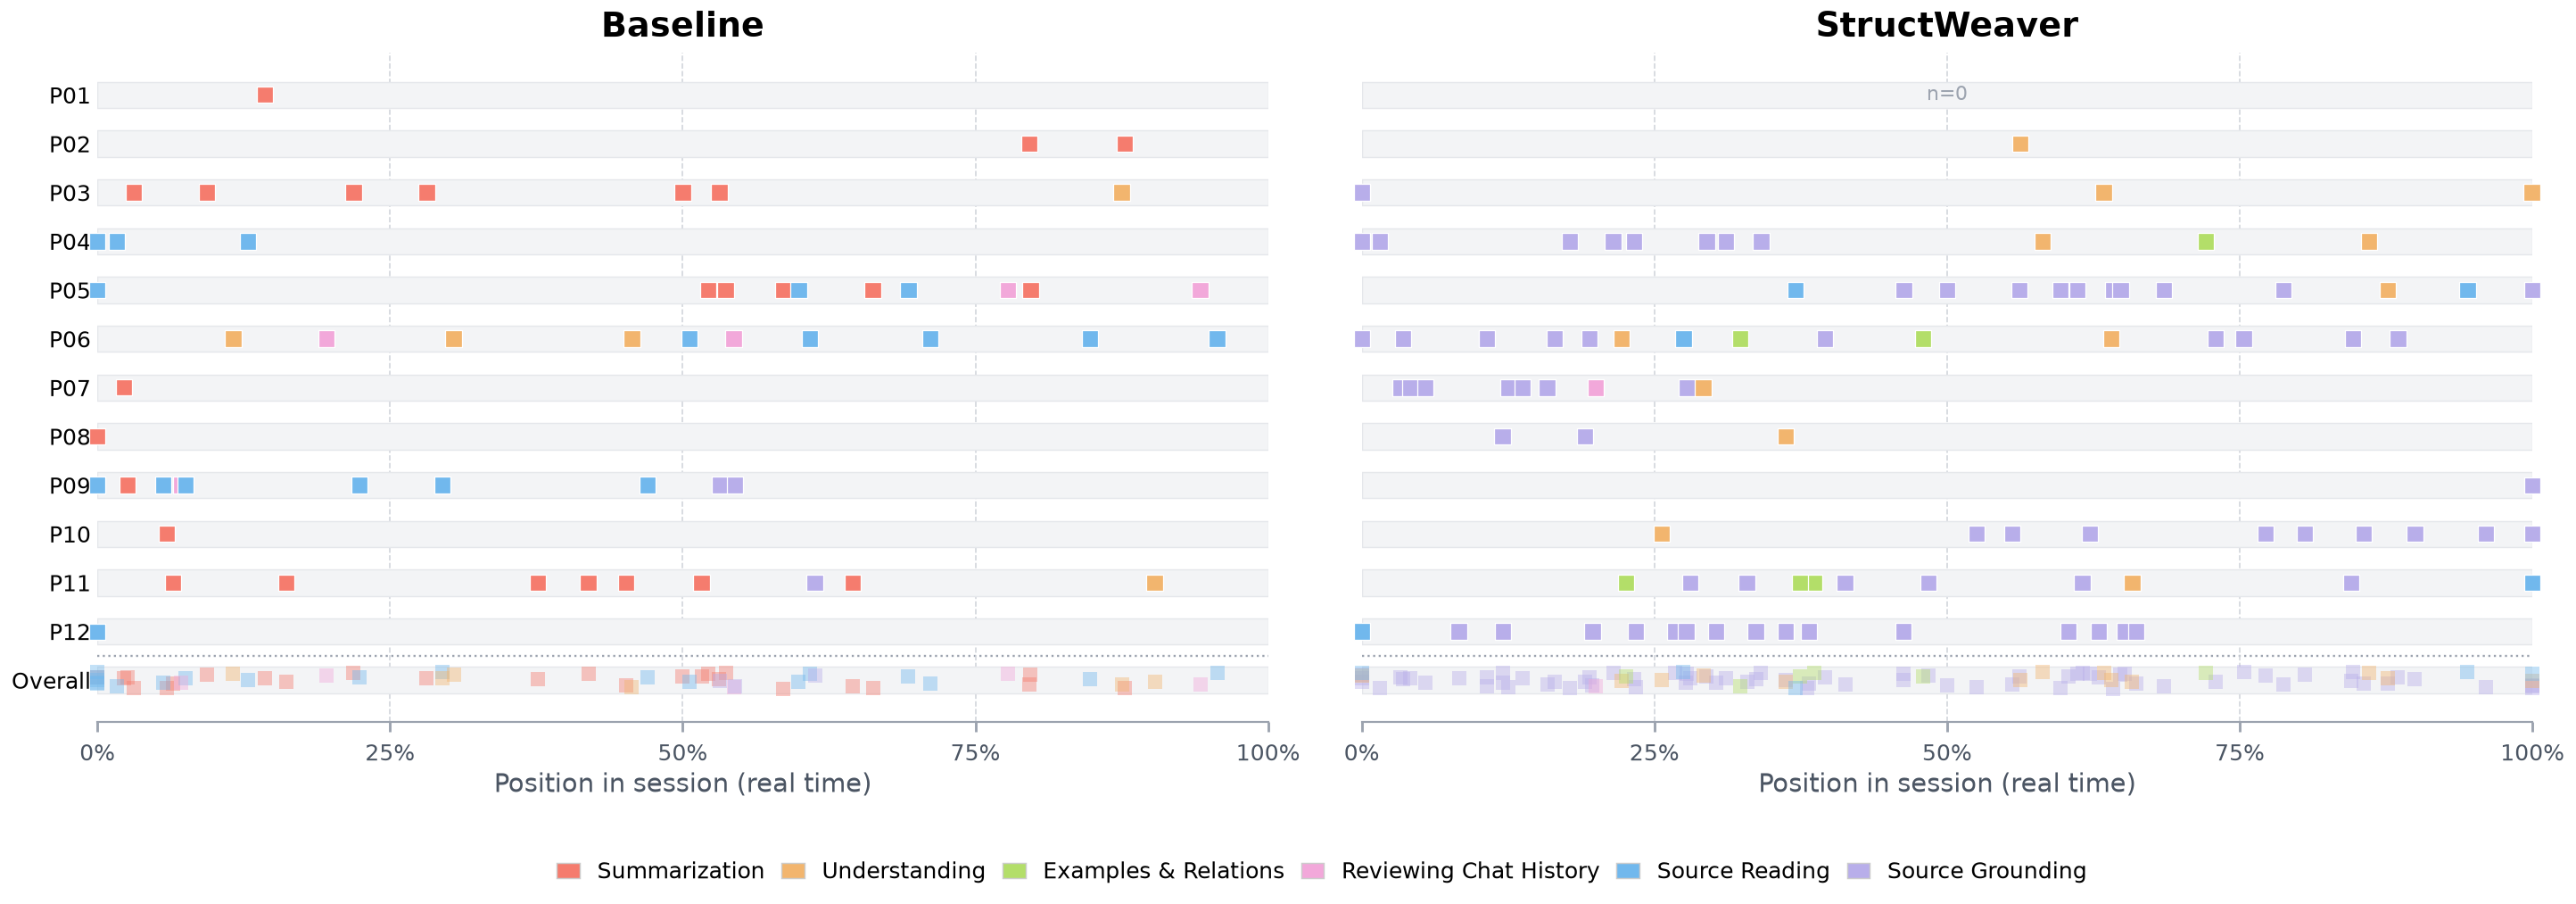
\includegraphics[width=\textwidth]{fig/compact_behavior_timeline.png}
\caption{Coded behaviors along the session timeline (real time, 0--100\%; $n=12$). Three authors coded screen recordings into six categories (Summarization, Understanding, Examples \& Relations, Chat Management, Source Reading, Source Grounding; definitions in \S\ref{sec:evaluation} Measures). Baseline is left, StructWeaver right. Each row is one participant; colored marks show approximate session progress when each behavior occurred. The bottom Overall row semi-transparently overlays all events.}
\label{fig:behavior-timeline}
\end{figure*}

\begin{figure*}[t]
\centering
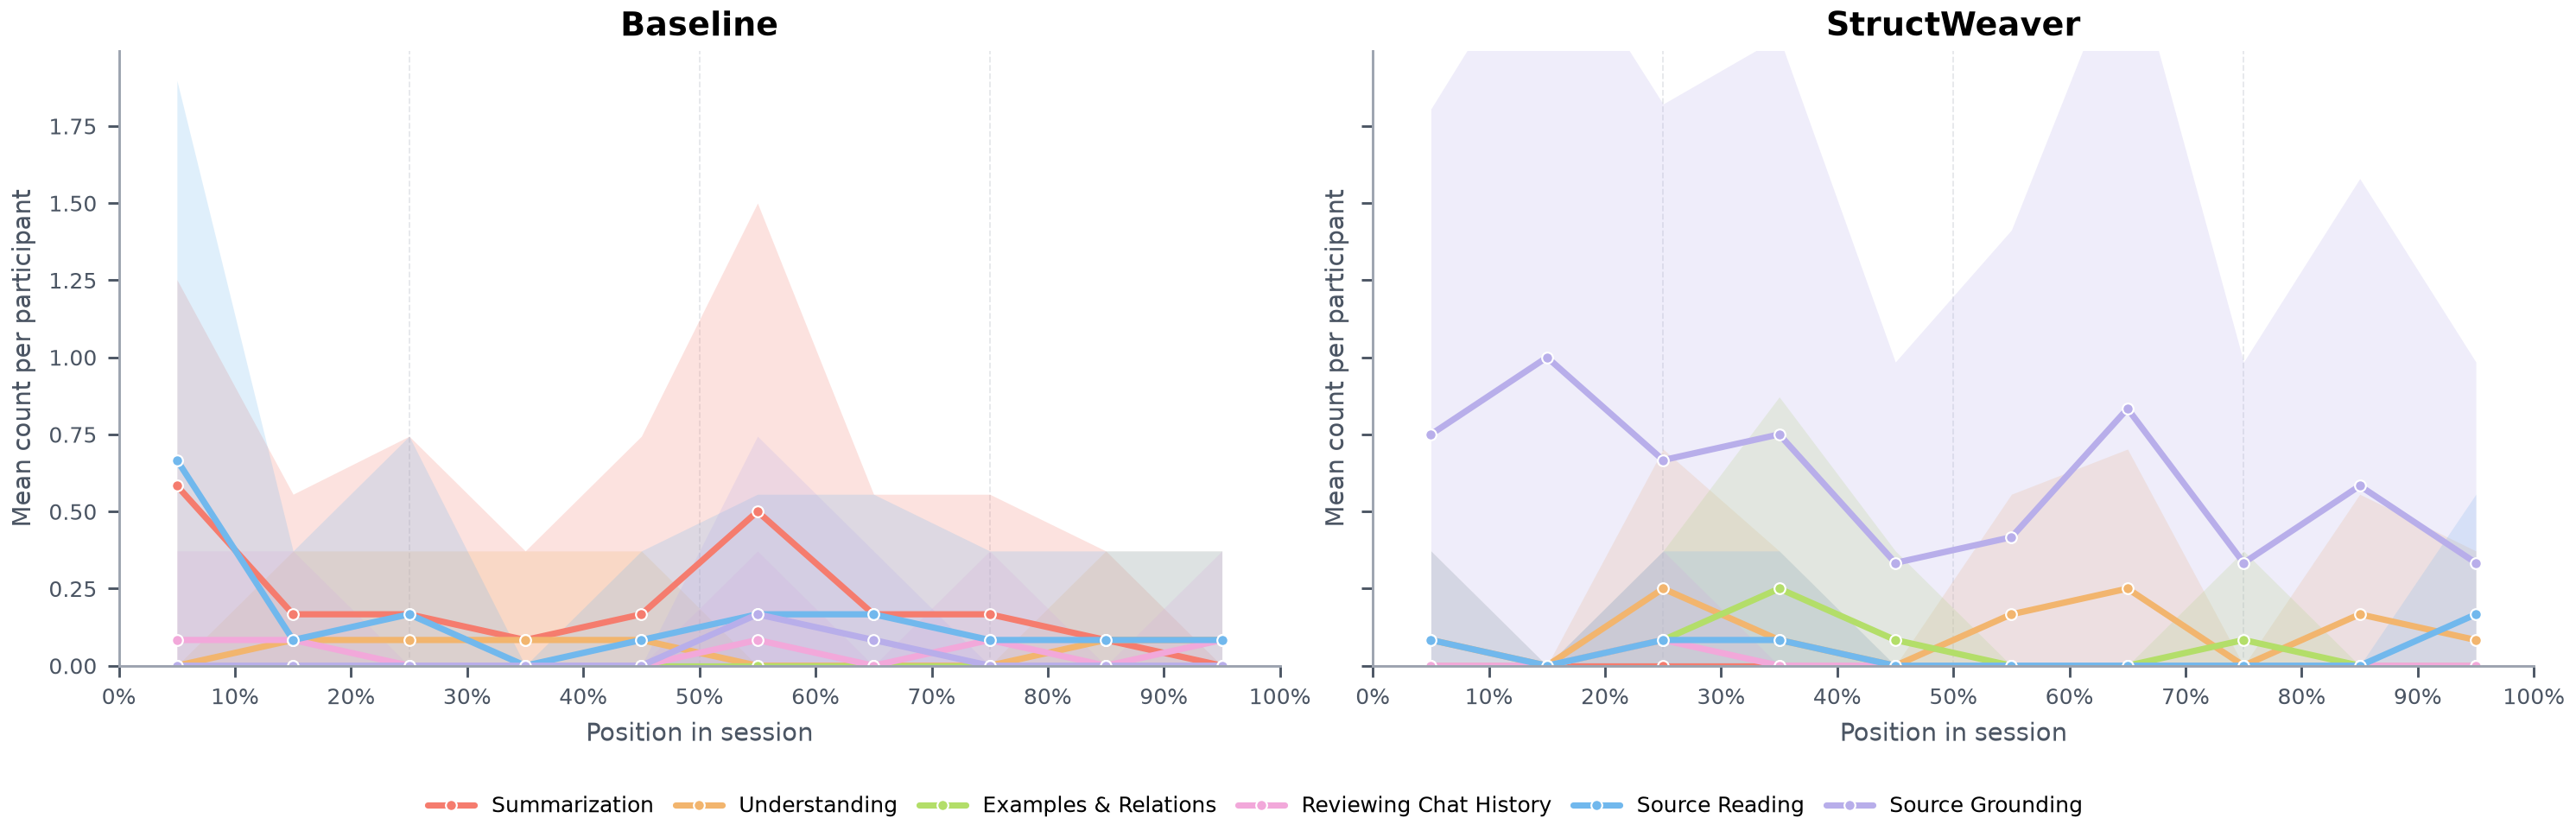
\includegraphics[width=\textwidth]{fig/compact_behavior_timeline_binned.png}
\caption{Behavior counts in 10\% session bins ($n=12$; same six-category coding as Figure~\ref{fig:behavior-timeline}). Solid lines show per-category means across participants; shaded bands indicate $\pm 1$ SD. Under StructWeaver, Source Grounding concentrates in the mid-to-late session; under Baseline, Summarization more often appears in the first half.}
\label{fig:behavior-binned}
\end{figure*}

\begin{table*}[t]
\centering
\caption{Wilcoxon signed-rank tests on coded behavior counts by category ($n=12$ paired participants). Values are mean counts per reading session (standard deviations in parentheses). Holm correction was applied across the six categories; total events per session is reported separately and was not included in the family-wise correction.}
\label{tab:behavior_stats}
\footnotesize
\setlength{\tabcolsep}{5pt}
\begin{tabular}{lcccccc}
\toprule
Category & Baseline $M$ ($SD$) & StructWeaver $M$ ($SD$) & $\Delta M$ & $d_z$ & $p$ & Holm $p$ \\
\midrule
Summarization & 2.08 (2.47) & 0.00 (0.00) & $-$2.08 & $-$0.84 & .004 & .023 \\
Understanding & 0.50 (0.90) & 1.08 (0.90) & $+$0.58 & 0.59 & .113 & .453 \\
Examples \& Relations & 0.00 (0.00) & 0.50 (1.00) & $+$0.50 & 0.50 & .250 & .562 \\
Chat Management & 0.42 (0.79) & 0.08 (0.29) & $-$0.33 & $-$0.38 & .375 & .562 \\
Source Reading & 1.58 (2.39) & 0.42 (0.67) & $-$1.17 & $-$0.50 & .188 & .562 \\
Source Grounding & 0.25 (0.62) & 6.00 (5.08) & $+$5.75 & 1.09 & .006 & .029 \\
\midrule
Total events & 4.83 (4.39) & 8.08 (6.01) & $+$3.25 & 0.48 & .112 & --- \\
\bottomrule
\end{tabular}
\end{table*}


We found source inspection became part of participants' ordinary reading process rather than a separate verification step. In the Baseline condition, participants often obtained an AI response first and then separately decided whether returning to the PDF was necessary. The StructWeaver condition instead allowed participants to move directly from an AI-generated gist node to its corresponding source passage. We observed participants repeatedly using these links while progressing through the paper, often without first expressing explicit doubt about the generated content. 
This suggests that returning to the source was not limited to explicit fact-checking episodes. Participants also inspected evidence while developing an initial interpretation of the paper. AI-generated gist therefore more often functioned as an entry point into the source rather than as an endpoint of the reading process.


\subsection{Gist--Verbatim Traversal Supported Interpretation Work}
\label{sec:interpretation-work}

Although behavioral logs show that participants returned to source evidence more frequently in the StructWeaver condition, screen recordings and interviews further revealed what participants did during these transitions. We observed three recurring practices: inspecting AI-generated interpretations against the source, using incomplete evidence correspondence as a cue for further inspection, and repairing mismatches between AI and author perspectives.

\subsubsection{Inspecting AI Interpretations against the Source}

Participants frequently used linked source passages to examine how AI-generated gist represented the original text. Rather than only determining whether an individual statement was correct, participants compared an abstraction with its source to understand what information had been selected, compressed, or emphasized. P11 described using the links to determine whether \textit{``these summarized keywords or claims are actually supported by real information in the original text.''} They further explained that being able to return to the corresponding passage increased their confidence in interpreting the generated structure. Gist nodes therefore provided an initial abstraction, while linked verbatim passages enabled participants to inspect how that abstraction related to the source.

This differed from the Baseline condition, where an AI-generated interpretation was often presented without an immediately visible connection to the text from which it was derived. In the StructWeaver condition, participants could inspect this relationship during reading and treat generated gist as an interpretation to examine rather than a completed summary to accept.

\subsubsection{Incomplete Evidence Correspondence Became a Cue for Further Inspection}

Participants also attended to cases in which the relationship between an AI-generated abstraction and source evidence appeared incomplete. P03 explained that when many generated points could be located in the original text, they considered those interpretations more reliable, whereas a point without clear source support could serve as a reminder that further verification was needed: \textit{``there is also another category without source support; its role is to remind the user to verify.''} Thus, source correspondence was useful not only when it confirmed an AI-generated claim. Weak or missing correspondence could itself direct participants' attention back to the source. Participants used these cases to identify when a generated abstraction appeared broader than the available evidence or when additional reading was necessary before accepting it.

This extended verification beyond asking whether an isolated statement was true or false. Participants also examined whether the generated gist adequately represented what the source was saying and whether information might have been omitted or over-compressed in the abstraction.

\subsubsection{Repairing Misalignment between AI and Author Perspectives}

Participants further used Gist--Verbatim traversal when the AI's organization of a paper did not match their interpretation of the author's argument. P11 contrasted the AI in the Baseline condition, where the model \textit{``comes with its own logic''} that readers could only passively follow, with the StructWeaver condition, where the generated structure could be compared directly with the original text. P03 similarly described treating the generated structure as a reference before returning to the paper to \textit{``judge for myself.''} These interactions allowed participants to coordinate three perspectives during reading: the organization proposed by the AI, the argument presented by the author, and their own developing interpretation. When these perspectives diverged, participants could return to the source to identify the mismatch rather than continuing along the AI-generated interpretation by default.

Taken together, these practices show that Gist--Verbatim correspondence served a broader role than citation retrieval. Participants used it to inspect how source information was compressed, detect where support appeared incomplete, and resolve differences between AI-generated organization and the source argument. The representation therefore made generated abstractions directly inspectable without requiring access to the model's internal reasoning process.

\subsection{StructWeaver Reduced Coordination Burden while Supporting Active Sensemaking}
\label{sec:cognitive-findings}

Questionnaire responses showed that the behavioral differences observed in the StructWeaver condition were accompanied by changes in participants' perceived cognitive experience. The StructWeaver condition reduced intrinsic and extraneous load while increasing germane load, suggesting that participants experienced less difficulty coordinating the reading workflow while devoting more effort to organizing and integrating the material itself.

\subsubsection{Lower Intrinsic and Extraneous Load}

Participants reported lower intrinsic load in the StructWeaver condition ($M=2.50$) than in the Baseline condition ($M=3.69$; $\Delta=-1.19$, $p=.026$, $d=-0.74$). Extraneous load similarly decreased from $M=3.44$ in the Baseline condition to $M=2.50$ in the StructWeaver condition ($\Delta=-0.94$, $p=.011$, $d=-0.87$). Item-level results provide additional context for these differences (Table~\ref{tab:survey_stats}). Participants reported less difficulty understanding document logic and causal relationships (Q1, $p=.016$), less need to repeatedly adjust the granularity of presented information (Q6, $p=.027$), and lower overall task effort (Q11, $p=.008$). Difficulty maintaining and processing information showed a marginal difference favoring the StructWeaver condition (Q3, $p=.059$), while Q2, Q4, Q5, and Q7 did not reach statistical significance.

\begin{table}[t]
\centering
\caption{Wilcoxon signed-rank tests for cognitive load questionnaire items ($n=12$). Items 1--6 and 11 are negatively framed (lower values indicate more favorable responses); items 7--10 are positively framed (higher values indicate more favorable responses).}
\label{tab:survey_stats}
\small
\begin{tabularx}{\linewidth}{c X c c}
\toprule
Q & Dimension & $p$ & Sig. \\
\midrule
1 & Difficulty understanding logic/causality & .016 & * \\
6 & Need to adjust content granularity & .027 & * \\
8 & Proactively organizing structure/summarizing & .049 & * \\
9 & Reading with concepts/questions in mind & .002 & ** \\
10 & Integrating scattered information & .006 & ** \\
11 & Overall task effort & .008 & ** \\
\midrule
3 & Difficulty maintaining/processing information & .059 & $\dagger$ \\
\multicolumn{4}{l}{\textit{Non-significant: Q2, Q4, Q5, Q7}} \\
\bottomrule
\end{tabularx}
\\[4pt]
\footnotesize{$^{*}\,p<.05$, $^{**}\,p<.01$, $\dagger$ marginal ($p<.06$).}
\end{table}

Participants' interviews help explain these differences. In the Baseline condition, participants described having to mentally coordinate information distributed across AI responses, the PDF, and their own emerging understanding. Returning to the source therefore required them to remember which part of a previous response they were examining and manually locate the corresponding text. P11 described this process as easier in the StructWeaver condition because they could \textit{``jump to the source with a click,''} which made them more willing to compare whether source evidence supported a generated claim. These accounts suggest that the reduction in perceived load was associated less with simplifying the paper itself than with reducing the effort required to reconstruct relationships among representations.


\subsubsection{Greater Germane Engagement with the Reading Material}

At the same time, participants reported higher germane load in the StructWeaver condition ($M=5.20$) than in the Baseline condition ($M=3.72$; $\Delta=+1.48$, $p<.001$, $d=1.85$). At the item level, participants reported more proactive organization and summarization of the material (Q8, $p=.049$), greater tendency to read with explicit concepts or questions in mind (Q9, $p=.002$), and greater integration of information distributed across the paper (Q10, $p=.006$). This pattern aligns with the behavioral observations above. Although StructWeaver reduced the effort involved in locating and reconnecting information, participants did not simply disengage from the reading task. Instead, their reported effort shifted toward activities such as organizing the paper's structure, comparing abstractions with evidence, and integrating information across passages. Participants similarly described the linked representation as helping them maintain the relationship between what the AI suggested and what the paper stated. This made it easier to continue an existing line of inquiry after inspecting the source instead of reconstructing conversational context each time they moved between AI and PDF. Taken together, the questionnaire and interview data suggest that StructWeaver changed how cognitive effort was allocated during AI-assisted reading: participants reported less burden from coordinating disconnected representations while engaging more strongly in activities associated with constructing and integrating an understanding of the paper.



\subsection{Summary Quality: Participant-Level Tests Were Conservative; Pooled-Triple Associations Were Annotator-Sensitive}
\label{sec:summary-quality-results}

As a descriptive quality guardrail, we computed Recall, Precision, and Hallucination for each participant's written summary under the StructWeaver and Baseline conditions using the author relational-triple procedure in \S\ref{sec:summary-eval} (per-participant scores in Table~\ref{tab:summary_quality}). The two annotators were authors---not external experts---and Table~\ref{tab:summary_quality} reports the triple coding used for primary analysis.

\paragraph{Participant level.}
Paired Wilcoxon signed-rank tests ($n=12$) showed no stable significant system advantage. Recall was slightly higher in the StructWeaver condition ($M=0.32$) than in the Baseline condition ($M=0.25$; $\Delta=+0.07$, $p=.233$), Precision was similarly higher ($M=0.91$ vs.\ $M=0.82$; $\Delta=+0.09$, $p=.625$), and Hallucination was lower ($M=0.04$ vs.\ $M=0.18$; $\Delta=-0.14$, $p=.063$, marginal). Directionally, StructWeaver showed slightly higher mean coverage and accuracy and slightly lower hallucination, but these paired differences were not stably significant.

\paragraph{Pooled triple level.}
Pooling the same author triple annotations across participants, contingency tables associating condition with accurate vs.\ inaccurate triples yielded $\chi^2=10.77$, $p=.001$ (Baseline: 69 accurate / 14 inaccurate; StructWeaver: 98 / 2), and associating condition with covered vs.\ uncovered cores yielded $\chi^2=6.46$, $p=.011$ (Baseline: 69 covered / 237 uncovered; StructWeaver: 98 / 208). Hallucination at this grain is the complement of the precision table and therefore shares the same $\chi^2$. When the second author applied the same triple procedure independently, pooled associations were not significant (precision/hallucination $\chi^2=0.03$, $p=.85$; recall $\chi^2=3.20$, $p=.074$), consistent with the annotator-strictness difference in \S\ref{sec:summary-eval}. Because triples are nested within participants, we treat pooled $\chi^2$ as descriptive of triple counts rather than as a substitute for the paired reader-level tests. Taken together, the conservative participant-level Wilcoxon results and the annotator-sensitive pooled associations suggest that the shift from summary consumption toward source grounding did not come with a clear, annotator-robust cost---or advantage---on headline coverage and factuality metrics.

\begin{table*}[t]
\centering
\caption{Per-participant summary quality under the StructWeaver and Baseline conditions ($n=12$), from the author relational-triple coding in \S\ref{sec:summary-eval} (not external experts). Cells are counts (hits/denominator). Recall denominators are core reference triples (22 or 29 depending on the assigned paper); Precision and Hallucination denominators are non-vague participant triples.}
\label{tab:summary_quality}
\footnotesize
\setlength{\tabcolsep}{4pt}
\begin{tabular}{lcccccc}
\toprule
Participant & SW Recall & SW Precision & SW Hallucination & BL Recall & BL Precision & BL Hallucination \\
\midrule
P01 & 2/22 & 2/3 & 1/3 & 3/29 & 3/6 & 3/6 \\
P02 & 5/22 & 5/6 & 0/6 & 12/29 & 11/11 & 0/11 \\
P03 & 7/22 & 7/7 & 0/7 & 4/29 & 4/4 & 0/4 \\
P04 & 13/29 & 13/13 & 0/13 & 8/29 & 6/6 & 0/6 \\
P05 & 11/29 & 11/11 & 0/11 & 7/29 & 6/8 & 2/8 \\
P06 & 13/22 & 13/13 & 0/13 & 10/22 & 9/9 & 0/9 \\
P07 & 11/29 & 11/11 & 0/11 & 3/22 & 4/4 & 0/4 \\
P08 & 2/29 & 2/5 & 1/5 & 6/22 & 7/10 & 3/10 \\
P09 & 8/29 & 8/8 & 0/8 & 10/29 & 6/7 & 1/7 \\
P10 & 9/22 & 9/9 & 0/9 & 11/29 & 7/7 & 0/7 \\
P11 & 11/29 & 11/11 & 0/11 & 6/22 & 6/6 & 0/6 \\
P12 & 6/22 & 6/6 & 0/6 & 0/29 & 0/4 & 4/4 \\
\bottomrule
\end{tabular}
\end{table*}

\subsection{Summary Evaluation Was More Reliable at the Triple Level}

Our summary evaluation also revealed substantial differences in annotation reliability depending on the granularity of the judgment. At the level of individual relational triples, the two author-annotators (the same authors who executed the triple procedure in \S\ref{sec:summary-eval}) were generally able to determine whether participant-generated content was supported by the paper. Hallucination judgments achieved 92.6\% raw agreement with Cohen's $\kappa=.535$, while agreement on correspondence to core reference points was $\kappa\approx.60$, depending on the annotation criterion. We nevertheless observed systematic differences between the two authors. One made significantly more hallucination judgments than the other (McNemar $\chi^2=6.67$, $p=.010$), indicating that even local factuality judgments depended partly on how strictly unsupported interpretations were defined---and helping explain why pooled-triple $\chi^2$ results differed when each author applied the same procedure independently. Agreement decreased substantially when judgments were made at the level of an entire participant summary. For whether a complete summary should be considered hallucinatory, raw agreement was 54.2\%, with Cohen's $\kappa=.083$. Thus, while the authors could more consistently assess whether individual triples were supported by the source, they frequently disagreed when characterizing the participant's overall interpretation. Given this difference, we rely primarily on triple-level annotations when using written summaries as a descriptive quality guardrail, keep participant-level Wilcoxon tests as the conservative comparison, and treat aggregate judgments about overall understanding more cautiously (Section~\ref{sec:discussion}).






% \section{Discussion}

% \subsection{From Trustworthy AI to Reversible Abstractions}

% Recent AI-assisted reading systems have largely focused on making AI outputs more trustworthy through provenance exposure, citation mechanisms, and calibration strategies. Our findings suggest a complementary perspective: trustworthiness alone may be insufficient if readers cannot naturally move between AI interpretations and source evidence. We argue that the underlying challenge is not simply evidence availability, but abstraction reversibility. AI-generated interpretations often become terminal outputs: readers can observe the result of AI understanding without being able to recover how that interpretation emerged from the original text. StructWeaver explores an alternative design direction. Rather than attaching provenance to completed outputs, it preserves relationships between abstractions and evidence throughout reading. This allows readers to continuously traverse between AI interpretations, source evidence, and their own evolving understanding instead of treating verification as a separate auditing step. More broadly, we suggest that future AI-assisted reading systems should move beyond asking whether evidence is visible, toward asking whether AI abstractions remain reversible throughout reading.

% \subsection{Verification Is a Capacity Problem Before It Is a Trust Problem}

% Existing discussions of AI overreliance often frame verification failures as problems of user attitudes, such as excessive trust or insufficient skepticism. Our findings suggest a different interpretation. Across both formative interviews and user studies, participants rarely described themselves as unwilling to verify AI outputs. Instead, they repeatedly encountered practical barriers: AI explanations, source documents, and their own interpretations existed in disconnected spaces that were difficult to coordinate simultaneously. StructWeaver did not necessarily make participants more skeptical of AI. Rather, it made verification easier to perform by preserving recoverable relationships among these representations. This shifts an important design question. Instead of asking, ``How do we motivate readers to verify AI outputs?'', future systems may ask, ``How do we increase readers' capacity to verify?'' This distinction may extend beyond academic reading. Similar challenges likely arise in policy analysis, educational materials, technical documentation, and other knowledge-intensive domains where AI increasingly acts as an intermediary interpreter rather than a direct information source.

% \subsection{AI-Assisted Reading Is Interpretation Work Rather Than Information Consumption}

% Our findings further suggest that AI-assisted reading may be better understood as interpretation work. Participants did not simply retrieve information from AI systems, nor did they merely fact-check isolated statements. Instead, they inspected how AI organized papers, identified potential omissions, and repaired mismatches between AI interpretations and author arguments. This distinction also helps differentiate StructWeaver from provenance-oriented systems. Provenance systems primarily support claim verification, whereas StructWeaver supports interpretation inspection. We therefore argue that AI-assisted reading should not only support access to evidence, but also externalize AI interpretations in ways that readers can inspect, challenge, and reorganize. In this sense, Gist--Verbatim alignment is not a mechanism for explaining model internals. Rather, it makes AI interpretations inspectable as relationships between abstractions and evidence. This perspective may also extend beyond academic papers to other forms of knowledge work, such as policy documents, technical reports, educational materials, and long-form organizational documents where AI increasingly acts as an interpretive intermediary.

% \subsection{Evaluating Reader Understanding Remains an Open Challenge}

% Our findings also reveal limitations in existing approaches to evaluating AI-assisted reading. As a quality guardrail, we evaluated participants' written summaries by converting them into triples and comparing them against author-generated core triples. Two authors first independently extracted core triples from each paper and used their intersection as reference concepts. Participant summaries were then converted into triples and independently evaluated for coverage and hallucination.

% Interestingly, agreement depended strongly on the evaluation granularity. At the triple level, inter-rater agreement was moderate to substantial. Hallucination judgments achieved 92.6\% raw agreement with Cohen's $\kappa = 0.535$, while core-point judgments achieved $\kappa \approx 0.60$ depending on annotation criteria. However, systematic asymmetries also emerged: one reviewer was significantly stricter when judging hallucinations (McNemar $\chi^2 = 6.67$, $p = .010$). At the summary level, agreement deteriorated substantially. For whether a summary should be considered hallucinatory, raw agreement dropped to 54.2\%, with Cohen's $\kappa = 0.083$. In other words, reviewers could often agree on local semantic units while disagreeing on the interpretation of a participant's overall understanding. We do not view this disagreement simply as annotation noise. Rather, it reflects a broader challenge in AI-assisted reading research: understanding does not always admit a single ground-truth representation.

% Readers may legitimately reorganize concepts, compress arguments, or construct intermediate inferences that are not explicitly stated in the source text. Consequently, it can be difficult to distinguish between correct interpretations, reasonable inferences, and hallucinations using correctness-oriented metrics alone. Interestingly, this difficulty mirrors the very problem that motivated our work. If AI-assisted reading inherently involves coordinating author arguments, AI-generated abstractions, and readers' own evolving explanations, then understanding itself may not be reducible to a single canonical representation. Future work may therefore require evaluation paradigms that better capture interpretive alignment and understanding construction, rather than relying solely on coverage- or correctness-based summary metrics.


\section{Discussion and Future Work}
\label{sec:discussion}

We discuss how StructWeaver supports reversible movement between AI-generated abstractions and source evidence, affects readers' capacity to verify AI interpretations, balances simple navigational scaffolds with richer relational structures, and reveals AI-assisted reading as a form of interpretation work.

\subsection{From Trustworthy Outputs to Reversible Abstraction}

AI-assisted reading systems commonly support verification by improving the quality or trustworthiness of generated outputs through citations, provenance information, or links to supporting source passages~\cite{scholarphi,papertrail,tabletale,kambhamettu2024traceabletextdeepeningreading}. These mechanisms help readers assess whether an AI-generated claim is grounded in the source. However, prior theories of sensemaking suggest that readers also need to move between representations at different levels of abstraction while preserving how those representations relate to one another~\cite{pirolli2005sensemaking,10.1145/169059.169209}. Our findings resonate with this distinction. Participants in the formative study could often access both AI-generated explanations and the original document, but verification became difficult when they had to reconstruct which source passages corresponded to earlier interpretations. In the evaluation, participants used StructWeaver's Gist--Verbatim links to move repeatedly between generated gist and source passages, allowing them to inspect how information had been compressed, identify incomplete support, and repair mismatches between AI and author perspectives.

We describe this property as \textit{reversible abstraction}. An abstraction is reversible when readers can move from a higher-level interpretation back to the source material from which it was constructed while retaining the relationship between the two. This differs from treating citations as references attached to a completed response. Instead, the abstraction--evidence relationship becomes part of the interaction structure that readers can revisit and extend~\cite{thuring1995hypermedia,hollan2000distributed}. StructWeaver instantiates this through decomposable gist units, explicit Gist--Verbatim links, and persistent interpretation paths.

This perspective suggests that AI-generated summaries may be more useful as intermediate representations than as final reading products~\cite{pirolli2005sensemaking}. Future work could investigate reversible abstraction in other forms of AI-generated structure, including outlines, argument maps~\cite{DWYER201016}, synthesized literature reviews~\cite{Synergi}, and representations that combine information from multiple sources. It also remains open how much of this structure should be generated automatically and how much readers should construct or revise as their understanding develops~\cite{vidsense}.

\subsection{Verification as Capacity rather than Skepticism}

Research on AI over-reliance often considers whether users trust generated outputs too readily or fail to verify them sufficiently~\cite{bucinca2021,romeo_conti2026,vered2023}. In reading tasks, fluent AI-generated explanations can further make unsupported or incomplete interpretations difficult to recognize~\cite{pastorino2025framing}. Our findings suggest that willingness to verify represents only part of this problem. Participants in the formative study rarely described verification as unnecessary; instead, they described difficulty sustaining it when AI responses, source documents, and their own emerging interpretations were distributed across disconnected interfaces~\cite{10.1145/169059.169209,papertrail}.

We observed a similar pattern in the evaluation. StructWeaver did not explicitly instruct participants to distrust AI or require them to verify particular outputs. Nevertheless, participants engaged in more source-grounding behavior. P11, for example, described becoming more willing to compare an AI-generated interpretation with the paper because the corresponding source could be reached directly. Participants also treated weak or incomplete Gist--Verbatim correspondence as a cue for further inspection~\cite{zhou2026improvinghumanverificationllm}. The cognitive-load results further showed lower intrinsic and extraneous load but higher germane load in the StructWeaver condition~\cite{sweller2011cognitive}. Rather than simply reducing effort, the system appeared to reduce the effort required to coordinate disconnected representations while allowing more effort to be directed toward organizing, comparing, and integrating information.

These observations suggest a distinction between the \textit{motivation} to verify and the \textit{capacity} to verify. Readers may already want to inspect an AI-generated interpretation but abandon verification when recovering the relevant evidence or conversational context becomes too costly~\cite{verification_burden_slr_iui,papertrail}. At the same time, lowering this cost may introduce a different form of reliance if readers begin to depend on system-generated alignment cues themselves~\cite{zhou2026improvinghumanverificationllm,bucinca2021}. Future research could examine how interaction support for verification should be combined with existing trust-calibration mechanisms, and when such scaffolding strengthens rather than substitutes for independent judgment.

\subsection{From Navigational Scaffolds to Richer Relations}

Visual diagramming for AI-assisted reading requires balancing the expressiveness of a representation with the effort required to understand and manipulate it. Mind maps provide a relatively lightweight visual grammar of nodes and branches~\cite{davies2011mind,hollan2000distributed}, whereas argument maps and semantic graphs can encode more explicit relational semantics through claims, premises, rebuttals, or typed edges~\cite{DWYER201016,A_Survey_on_Knowledge_Graphs,graphologue}. StructWeaver adopts a tree-based workspace not because readers' understanding is assumed to be inherently hierarchical, but because inquiry during AI-assisted reading often begins from a local point of interest and develops incrementally through follow-up questions and branching exploration~\cite{pirolli2005sensemaking,forage_chi26}. A simple hierarchy makes these paths visible while requiring relatively little additional representational knowledge from readers who are already working to understand an unfamiliar document. Seen through the lens of visual diagramming, this is a deliberate design trade-off: StructWeaver prioritizes recoverable gist--evidence and inquiry paths over the expressiveness of a free-form canvas. Because the node workspace scrolls vertically, moving deeper into a branch largely proceeds by scrolling down the page; readers therefore experience depth as a linear gist sequence rather than as spatial clutter on a wide canvas.

The tree in StructWeaver therefore acts as an initial scaffold rather than a fixed model of sensemaking. Readers can reorganize nodes and connect information across branches as their understanding develops, allowing the workspace to move beyond its original parent--child organization~\cite{liquidtext,graphologue}. We view this as \textit{progressive relational complexity}: starting with relations that are easy to perceive and recover, and introducing richer relationships as readers acquire enough context to make them useful~\cite{pirolli2005sensemaking,vidsense,10.1145/169059.169209}.

This trade-off is also visible in systems that provide richer spatial and multilevel representations. \textit{Sensecape}, for example, supports exploration through hierarchy views, semantic zoom, and semantic dive~\cite{sensecape}, but its study also reported that some participants found the hierarchy complex or overwhelming and associated the system with a learning curve. Prior work similarly notes that organizing information across abstraction levels or nonlinear spatial layouts can itself introduce additional sensemaking and interaction demands~\cite{pirolli2005sensemaking,liquidtext}. StructWeaver occupies a different point in this design space by keeping gist, source evidence, and subsequent inquiry within a stable visual workspace whose primary reading motion is vertical scroll along a branch. Remaining scalability concerns therefore lie less in downward depth---which largely reads as linear gist---and more in lateral branching, very long documents with many parallel inquiry paths, and the effort of reorienting across collapsed or reorganized subtrees. Future research could investigate when readers benefit from introducing additional relation types or spatial freedom, and whether the appropriate level of representational complexity changes with domain expertise, task familiarity, or the maturity of the reader's understanding.

\subsection{AI-Assisted Reading as Interpretation Work}

AI-assisted reading involves more than retrieving information or checking whether individual statements are factually supported. Participants used StructWeaver to examine how AI organized a paper, determine which source content had been compressed into particular gist units, notice potentially incomplete abstractions, and resolve differences between the AI's organization and the author's argument. These activities resemble interpretation work~\cite{supporting_or_hindering_chi26,thought_exchanges_iui,abstractexplorer}, in which readers continuously negotiate among what the source states, how an AI system represents it, and how they themselves understand the material.

This perspective also distinguishes Gist--Verbatim alignment from conventional provenance support~\cite{papertrail,kambhamettu2024traceabletextdeepeningreading}. A Gist--Verbatim link does not reveal the internal reasoning process of the language model or explain why a particular sentence was generated. Instead, it externalizes a relationship between an AI-generated interpretation and the source material against which that interpretation can be inspected~\cite{hollan2000distributed,pirolli2005sensemaking}. Participants' use of source traversal for omission detection and misalignment repair illustrates this distinction. Their question was often not only whether a claim was supported, but whether the generated abstraction represented an appropriate way of understanding the author's argument.

This interpretation-oriented view also has implications for evaluation. In our summary evaluation, annotators agreed more strongly when judging individual semantic relations than when evaluating a participant's summary as a whole. Local relations could often be compared with specific evidence, whereas overall interpretations involved judgments about acceptable compression, reorganization, and inference. This is consistent with prior work showing that readers can produce different but still reasonable organizations of the same material~\cite{abstractexplorer}. Consequently, summary-level correctness may not provide the same clear ground truth as local factual support~\cite{nenkova-passonneau-2004-evaluating}.

Future evaluations of AI-assisted reading could therefore complement coverage and factuality measures with measures of \textit{interpretive alignment}: whether readers can recover how an AI interpretation relates to the source, recognize plausible alternative interpretations, and construct explanations that remain grounded while reflecting their own reading goals. Longitudinal work could further examine whether persistent interpretation structures improve later recall, transfer, and the ability to resume complex reading after interruption~\cite{garden_of_papers,Synergi,threddy}.




% \section{Conclusion}

% AI-assisted reading is often framed as a problem of trust, factual correctness, or hallucination. However, our findings suggest that a more fundamental challenge lies in how AI-generated abstractions are represented throughout reading. Although AI systems increasingly provide personalized summaries and provenance information, readers still struggle to reconnect AI interpretations with author arguments and their own evolving understanding.

% In this paper, we reframed AI-assisted reading as a problem of reversible abstraction and introduced StructWeaver as an instantiation of Gist--Verbatim alignment. Rather than treating verification as an additional auditing step, StructWeaver preserves recoverable paths among AI interpretations, source evidence, and readers' evolving understanding. Through formative studies and a paired within-subject evaluation, we found that this alignment reconfigured AI-assisted reading from summary consumption toward interpretation work, enabling readers to inspect, challenge, and reorganize AI-generated interpretations during reading.

% More broadly, our work suggests a shift in how future AI-assisted reading systems may be designed. The goal may not be to produce increasingly trustworthy AI outputs, but to ensure that AI-generated abstractions never become irreversible. Instead of asking readers to trust, distrust, or repeatedly verify AI after the fact, future systems may support understanding by preserving traversable relationships among author arguments, AI interpretations, and readers' own explanations.


\section{Conclusion}

In this paper, we present StructWeaver, an interactive AI-assisted reading system that supports readers in traversing between AI-generated gist and source evidence. It achieves this through decomposable gist representations, explicit Gist--Verbatim correspondence, and persistent interpretation paths that preserve relationships among AI interpretations, author arguments, and readers' evolving understanding. Our formative study identified key breakdowns in maintaining these relationships during long-form AI-assisted reading, informing the design of StructWeaver. A within-subjects user study further showed that StructWeaver shifted reading from repeated summary consumption toward source-grounded interpretation, while reducing coordination burden and supporting more active organization and integration of information. Our work highlights reversible abstraction as a design direction for future AI-assisted reading systems that seek to make AI-generated interpretations more inspectable, recoverable, and grounded in source materials.




\bibliographystyle{ACM-Reference-Format}
\bibliography{sample-base,related_work,screening_corpus}

\appendix

\section{Study Materials}
\label{appendix:study-materials}

\subsection{Main Task Papers}
Each participant read one of the following CHI papers under StructWeaver and the other under Baseline (assignment counterbalanced with interface order):
\begin{itemize}[leftmargin=*, noitemsep]
  \item \textit{Why Johnny Can't Prompt: How Non-AI Experts Try (and Fail) to Design LLM Prompts}~\cite{Zamfirescu-Pereira}
  \item \textit{Synthetic Lies: Understanding AI-Generated Misinformation and Evaluating Algorithmic and Human Solutions}~\cite{synthetic_lies}
\end{itemize}

\subsection{Eligibility Screening Corpus}
Prior to the main tasks, we used an HCI-oriented paper pool to confirm that participants could engage in AI-assisted long-form reading. The pool emphasized dialogue agents, sensemaking, scholarly synthesis, visual programming, and related HCI topics. Titles included:
\begin{itemize}[leftmargin=*, noitemsep]
  \item Towards Lifelong Dialogue Agents via Timeline-based Memory Management~\cite{lifelong_dialogue_agents}
  \item Selenite: Scaffolding Online Sensemaking with Comprehensive Overviews Elicited from Large Language Models~\cite{selenite}
  \item Structuring Knowledge with Cognitive Maps and Cognitive Graphs~\cite{PEER202137}
  \item Spellburst: A Node-based Interface for Exploratory Creative Coding with Natural Language Prompts~\cite{spellburst}
  \item Synergi: A Mixed-Initiative System for Scholarly Synthesis and Sensemaking~\cite{Synergi}
  \item The Story in the Notebook: Exploratory Data Science using a Literate Programming Tool~\cite{story_in_notebook}
  \item The evaluation of argument mapping as a learning tool: Comparing the effects of map reading versus text reading on comprehension and recall of arguments~\cite{DWYER201016}
  \item Threddy: An Interactive System for Personalized Thread-based Exploration and Organization of Scientific Literature~\cite{threddy}
  \item Towards an instrument for measuring sensemaking and an assessment of its theoretical features~\cite{alsufiani_sensemaking_instrument}
  \item mage: Fluid Moves Between Code and Graphical Work in Computational Notebooks~\cite{mage}
  \item PaperWeaver: Enriching Topical Paper Alerts by Contextualizing Recommended Papers with User-collected Papers~\cite{paperweaver}
  \item Patterns of Hypertext-Augmented Sensemaking~\cite{hypertext_augmented_sensemaking}
  \item Positional Control in Node-Based Programming~\cite{positional_control}
  \item Opening up the black box of scholarly synthesis: Intermediate products, processes, and tools~\cite{qian_scholarly_synthesis}
  \item Relatedly: Scaffolding Literature Reviews with Existing Related Work Sections~\cite{relatedly}
  \item ScholarMate: A Mixed-Initiative Tool for Qualitative Knowledge Work and Information Sensemaking~\cite{scholarmate}
  \item Leveraging Large Language Models for Realizing Truly Intelligent User Interfaces~\cite{oelen_llm_iui}
  \item A Similarity Measure for Comparing Conversational Dynamics~\cite{condyns}
  \item Closing the Loop: Learning to Generate Writing Feedback via Language Model Simulated Student Revisions~\cite{nair_closing_loop}
  \item Developing a Model of Distributed Sensemaking: A Case Study of Military Analysis~\cite{wheat_distributed_sensemaking}
  \item Rapsai: Accelerating Machine Learning Prototyping of Multimedia Applications through Visual Programming~\cite{rapsai}
  \item Effects of Implicit Sharing in Collaborative Analysis~\cite{goyal_implicit_sharing}
  \item eRevise+RF: A Writing Evaluation System for Assessing Student Essay Revisions and Providing Formative Feedback~\cite{erevise_rf}
  \item Graphologue: Exploring Large Language Model Responses with Interactive Diagrams~\cite{graphologue}
  \item Interactive Visual Analytics for Sensemaking with Big Text~\cite{big_text_sensemaking}
\end{itemize}

\section{Illustrative Reading Walkthrough}
\label{appendix:walkthrough}

The following vignette reconstructs one participant's session (P08; materials-science graduate) from screen recordings and post-task debrief. P08 read \textit{Why Johnny Can't Prompt} under Baseline and \textit{Synthetic Lies} under StructWeaver (counterbalanced assignment). Coded behavior counts for P08 appear in Table~\ref{tab:behavior_stats}. This case is illustrative rather than representative: P08 showed strong summary-quality gains under StructWeaver despite relatively few source-grounding actions, consistent with a \textit{plausible-then-skip} verification pattern observed in debrief.

\subsection{Baseline: \textit{Why Johnny Can't Prompt}}

\paragraph{Workflow.}
P08 opened the assigned PDF in the viewer and provided the paper to ChatGPT, then requested a plain-language overview organized around background, problem, methods, findings, and contributions. The model returned a multi-section summary that made the paper's scope legible at a high level.

\paragraph{Linear follow-up.}
P08 continued in the same chat thread with clarifying questions---for example, what \textit{probe} meant in the paper's HCI sense, why BotDesigner was described as a ``half-finished'' research tool rather than a polished product, and how non-experts ``opportunistically'' patched prompts after each bot failure. Each answer extended the conversation downward, mixing accurate explanations with paraphrases that were increasingly detached from specific source sentences.

\paragraph{Verification friction.}
When the model attached citation-style links or page references, P08 clicked them expecting sentence-level anchors. The links opened the PDF viewer but did not highlight the supporting passage, so P08 could not tell which sentence justified a claim. After a few attempts, P08 stopped following links and relied on whether the explanation ``sounded plausible.'' Screen recordings coded zero source-grounding actions for this session.

\paragraph{Coordination cost and summary.}
As the thread grew, P08 scrolled repeatedly to recover earlier explanations before continuing. P08 later reported that much of the reading felt ``forgotten'' when starting the closed-book summary. The written summary captured several high-level themes but included unsupported elaborations (Precision $=0.30$; Hallucination rate $=0.40$ for this participant under Baseline; Table~\ref{tab:summary_quality}).

\subsection{StructWeaver: \textit{Synthetic Lies}}

\paragraph{Entry through gist structure.}
Facing a long COVID-misinformation paper outside her primary domain, P08 first scanned top-level gist nodes to learn \textit{how the study was done} rather than reading linearly from the PDF. Subordinate nodes on the right listed concrete steps---collecting human-written false claims, extracting narrative elements as prompts, generating paired GPT-3 outputs, and comparing detection performance---which P08 browsed before selecting branches of interest.

\paragraph{Gist--verbatim traversal.}
When a gist node noted differences in \textit{language style} between human- and AI-written misinformation, P08 opened the linked verbatim panel and encountered psycholinguistic terms (e.g., categorical--dynamic index [CDI], clout, authentic tone). Unfamiliar with CDI, P08 asked a path-scoped question on that node; the response explained the construct using the local gist and aligned source sentences. P08 then returned to the active branch by clicking the verbatim or gist node rather than searching a long chat log.

\paragraph{Alternating overview and depth.}
P08 alternated between map-level overview (confirming where she was in the argument) and localized depth (reading evidence for one sub-claim). Debrief responses characterized this as ``getting the direction right first'' and then selectively checking points she did not understand. Screen recordings coded two source-grounding actions and one node-level understanding request for this session---fewer than some participants, but aligned with P08's stated selective verification habit. At the time of the study, StructWeaver's precomputed structure covered the abstract and introduction of this paper; participants could still open the full PDF when needed.

\paragraph{Outcomes.}
Relative to Baseline, P08 reported lower intrinsic and extraneous load, higher germane load, and produced a summary with perfect precision and no coded hallucinations (Table~\ref{tab:summary_quality}). This improvement co-occurred with structured gist--verbatim access rather than with intensive line-by-line verification, highlighting that outcome gains and verification intensity can diverge at the participant level.

\subsection{Contrast}

Across the two sessions, the same reader shifted from summary-first consumption with chat-managed clarification (Baseline) to gist-first exploration with recoverable paths back to evidence (StructWeaver). Baseline separated AI paraphrase, PDF location, and memory; StructWeaver linked abstractions to verbatim nodes and preserved branch context for follow-up questions. The vignette therefore instantiates the aggregate behavioral pattern in \S\ref{sec:findings}: decreased summarization/compression, increased (though not uniformly intensive) source grounding, and reduced coordination cost when returning to the text.

\section{Core System Algorithms}
\label{sec:appendix-algorithms}

This appendix provides pseudocode for the Gist--Verbatim construction pipeline referenced in Section~\ref{sec:implementation}. Raster formula fragments from the Word draft are preserved under \texttt{fig/word/} (media \texttt{image9}--\texttt{image146}).

\subsection{Paragraph-Level Gist Generation and Decomposition}

For each paragraph $p$ in the source document:
\begin{enumerate}[leftmargin=*, noitemsep]
\item Segment the document into paragraphs while preserving the existing Markdown heading hierarchy.
\item Prompt DeepSeek-V4-Flash to generate a localized gist for $p$.
\item Decompose the gist into sentence-level units $\{g_1, \ldots, g_n\}$ following the model's bullet or sentence structure.
\item Split $p$ into source sentences $\{s_1, \ldots, s_m\}$ in document order.
\item Run order-preserving embedding--DP alignment (Algorithm~\ref{alg:alignment}) to link each $s_i$ to exactly one $g_j$.
\item Attach verbatim nodes for matched sentences under their governing gist nodes in the node graph.
\end{enumerate}

\subsection{Order-Preserving Gist--Sentence Alignment}

Given $m$ source sentences $\{s_1, \ldots, s_m\}$ and $n$ AI-generated gist units $\{g_1, \ldots, g_n\}$ within a paragraph, StructWeaver encodes each sentence and gist unit in a shared embedding space and computes a similarity matrix $W \in \mathbb{R}^{m \times n}$, where $W_{i,j} = \cos(\mathrm{embed}(s_i), \mathrm{embed}(g_j))$. The system then finds an order-preserving assignment that maps every source sentence to exactly one gist unit while maximizing total similarity. One gist unit may govern multiple contiguously ordered sentences (one-to-many extension), but source order is preserved globally.

Dynamic programming state $D[i][j]$ stores the best score for aligning the first $i$ sentences with the first $j$ gist units. Transitions include: (1) \textit{match}: assign $s_i$ to $g_j$; (2) \textit{extend}: assign $s_i$ to the same $g_j$ as $s_{i-1}$; (3) \textit{skip\_i} / \textit{skip\_j}: advance one sequence with a gap penalty when no confident match exists.

\begin{algorithm}[h]
\caption{Order-Preserving Gist--Sentence Alignment}
\label{alg:alignment}
\begin{algorithmic}[1]
\Require Source sentences $s_{1..m}$, gist units $g_{1..n}$, embedding function $\mathrm{embed}(\cdot)$, minimum similarity $\tau$
\Ensure Assignment mapping each sentence index to a gist index
\State Compute $W_{i,j} \gets \cos(\mathrm{embed}(s_i), \mathrm{embed}(g_j))$ for all $i,j$
\State Initialize $D[0][0] \gets 0$; all other $D[i][j] \gets -\infty$
\For{$i = 0$ to $m$}
 \For{$j = 0$ to $n$}
 \If{$i > 0$}
 \State $D[i][j] \gets \max(D[i][j], D[i-1][j] - \gamma_i)$ \Comment{skip sentence}
 \EndIf
 \If{$j > 0$}
 \State $D[i][j] \gets \max(D[i][j], D[i][j-1] - \gamma_j)$ \Comment{skip gist unit}
 \EndIf
 \If{$i > 0$ and $j > 0$ and $W_{i,j} \ge \tau$}
 \State $D[i][j] \gets \max(D[i][j], D[i-1][j-1] + W_{i,j})$ \Comment{new match}
 \State $D[i][j] \gets \max(D[i][j], D[i-1][j] + W_{i,j})$ \Comment{extend same gist}
 \EndIf
 \State Record backpointer for best transition at $(i,j)$
 \EndFor
\EndFor
\State Trace backpointers from $(m,n)$ to recover sentence-to-gist pairs
\State \Return grouped assignment $\{s_i : f(i)=j\}$ for each gist unit $g_j$
\end{algorithmic}
\end{algorithm}

For each gist unit $g_j$, StructWeaver creates verbatim nodes for all sentences $s_i$ such that $f(i)=j$ and attaches them under the corresponding gist node in the node graph.

\section{Path-Based Context Construction}
\label{appendix:context}

To preserve local reasoning context while avoiding the accumulation of irrelevant conversational history, StructWeaver constructs prompts from the node graph rather than from a linear transcript.

Given a target question node $q$, the system first identifies the user-selected reasoning path and then traverses connected nodes in depth-first order. Cross-links are treated as additional subtrees. A visited set prevents infinite loops when cyclic structures are present.

The resulting ordered sequence of nodes is serialized into a prompt and sent to the LLM. This procedure allows readers to explicitly determine which concepts, questions, and prior interpretations should influence subsequent responses.

\begin{algorithm}[t]
\caption{Path-Based Context Construction}
\label{alg:context}
\small
\begin{algorithmic}[1]

\Require Target node $q$
\Ensure Ordered context sequence $C$

\State $C \leftarrow [\,]$
\State $Visited \leftarrow \varnothing$

\Procedure{DFS}{$n$}

 \If{$n \in Visited$}
 \State \Return
 \EndIf

 \State $Visited \leftarrow Visited \cup \{n\}$

 \State Append $n$ to $C$

 \ForAll{$child \in Children(n)$}
 \State \Call{DFS}{$child$}
 \EndFor

 \ForAll{$link \in CrossLinks(n)$}
 \State \Call{DFS}{$link$}
 \EndFor

\EndProcedure

\State $Root \leftarrow$ reasoning root associated with $q$

\State \Call{DFS}{$Root$}

\State \Return $C$

\end{algorithmic}
\end{algorithm}

\section{Structure-Aware Summary Quality Comparison Between StructWeaver and Baseline Conditions}

Inspired by evaluation practices in natural language processing, such as ROUGE for summarization~\cite{lin-2004-rouge} and relation-based Basic Elements~\cite{hovy-etal-2006-automated}, we adopted a structure-aware evaluation of participant-written summaries (see also \S\ref{sec:summary-eval} and Table~\ref{tab:summary_quality}).

Two authors---not external experts---independently extracted core relational triples from each source introduction (29 for \textit{Synthetic Lies}; 22 for \textit{Why Johnny Can't Prompt}) and retained their intersection as the reference set. Participant summaries were segmented into semantic units, converted into triples, and scored blind to system condition for coverage and factual support under the same triple procedure as \S\ref{sec:summary-eval}.

We defined the following evaluation metrics:

\begin{itemize}[noitemsep, leftmargin=*]

\item Recall ($\mathcal{R}$): proportion of core reference triples covered by the participant summary.
$$
\mathcal{R} = \frac{\text{Covered core triples}}{N_{\text{core}}}
$$

\item Precision ($\mathcal{P}$): proportion of participant-generated triples that accurately reflected the source paper.
$$
\mathcal{P} = \frac{\text{Accurate participant triples}}{N_{\text{user,total}}}
$$

\item Hallucination Rate ($\mathcal{H}$): proportion of participant-generated triples containing unsupported or inaccurate information.
$$
\mathcal{H} = \frac{\text{Unsupported or inaccurate triples}}{N_{\text{user,total}}}
$$

\end{itemize}

Paired Wilcoxon signed-rank tests on per-participant rates ($n=12$) yielded: Recall $p=.233$, Precision $p=.625$, Hallucination $p=.063$.

\section{Survey Items on AI Reading Habits and Verification Tendencies}

Participants responded to the following items on a 7-point Likert scale 
(1 = Strongly Disagree, 7 = Strongly Agree). 
Reverse-coded items are marked with (R).

\subsection*{Dimension 1: Verification Habits}
\begin{enumerate}[label=\arabic*.]
 \item I actively verify whether the information provided by AI is correct. 
 \item If the AI’s answer appears reasonable, I usually do not check it further. (R)
 \item I habitually cross-check AI’s responses with original sources (e.g., papers, news articles, textbooks).
\end{enumerate}

\subsection*{Dimension 2: Dependency Level}
\begin{enumerate}[label=\arabic*.]
 \item When reading, I tend to rely more on AI summaries than on reading the full text myself.
 \item If the AI does not provide an answer, I find the reading task more difficult.
\end{enumerate}

\subsection*{Dimension 3: Trust Attitude}
\begin{enumerate}[label=\arabic*.]
 \item I usually believe that the information provided by AI is accurate.
 \item I remain skeptical of AI’s responses until they are verified. 
\end{enumerate}

\subsection*{Dimension 4: Usage Style}
\begin{enumerate}[label=\arabic*.]
 \item I adjust my reading focus based on the answers given by AI. 
 \item I often treat AI outputs as cues rather than final conclusions. 
\end{enumerate}

\section{Cognitive Load Questionnaire (Long-text Reading Version)}

Participants responded to the following items on a 7-point Likert scale 
(1 = Strongly Disagree, 7 = Strongly Agree), based on their experience during the task.

\subsection*{Dimension 1: Intrinsic Load}
Reflects the inherent complexity and difficulty of the task.
\begin{enumerate}[label=\arabic*.]
 \item I found it difficult to understand the logical chains and causal relations in the text.
 \item The number of concepts and the amount of information in this long text felt overwhelming.
 \item Holding and processing all the information in mind at the same time was mentally demanding.
\end{enumerate}

\subsection*{Dimension 2: Extraneous Load}
Reflects additional burden introduced by AI outputs or the interface.
\begin{enumerate}[label=\arabic*.]
 \setcounter{enumi}{3}
 \item The AI outputs made it harder for me to judge which information was reliable.
 \item The way the interface or tools presented information distracted my attention.
 \item The level of detail in the AI’s content (too coarse or too fine-grained) required additional effort to adjust.
\end{enumerate}

\subsection*{Dimension 3: Germane Load}
Reflects constructive effort that contributes to knowledge building.
\begin{enumerate}[label=\arabic*.]
 \setcounter{enumi}{6}
 \item I tried to connect the new information in the text with my prior knowledge.
 \item I actively organized the structure and summarized key points during reading.
 \item Approaching the text with guiding concepts or questions helped me understand the content more effectively.
 \item I made an effort to integrate scattered information into a coherent knowledge network.
\end{enumerate}

\subsection*{Dimension 4: Total Load}
Reflects the overall perceived effort of the task.
\begin{enumerate}[label=\arabic*.]
 \setcounter{enumi}{10}
 \item Overall, I found this task mentally effortful.
\end{enumerate}


\section{System Impact Evaluation Questionnaire}

Participants responded to the following items on a 7-point Likert scale 
(1 = Strongly Disagree, 7 = Strongly Agree), based on their experience of using the system.

\subsection*{Dimension 1: Understand (Items 1--3)}
\begin{enumerate}[label=\arabic*.]
 \item Using this system helped me better understand the overall logic of the long text.
 \item The system supported me in integrating scattered information into a more organized knowledge structure.
 \item I felt that the system improved my grasp of key concepts in the text.
\end{enumerate}

\subsection*{Dimension 2: Verify (Items 4--6)}
\begin{enumerate}[label=\arabic*.]
 \setcounter{enumi}{3}
 \item The system made me pay more attention to the authenticity and sources of information.
 \item Through the linkage between original text and AI-generated nodes, this system made it easier for me to notice potential errors or hallucinations in AI outputs.
 \item After using the system, I became more willing to actively open original-text nodes to verify AI outputs at the source.
\end{enumerate}

\subsection*{Dimension 3: Re-understand (Items 7--9)}
\begin{enumerate}[label=\arabic*.]
 \setcounter{enumi}{6}
 \item I believe that this reading approach will help me in handling complex materials in the future.
 \item The system encouraged me to actively ask questions and explore during reading.
 \item I feel that this approach may change how I rely on AI in future reading (e.g., by trusting more, being more cautious, or paying greater attention to combining AI outputs with the original text).
\end{enumerate}

\subsection*{Dimension 4: Acceptance and Recommendation}
\begin{enumerate}[label=\arabic*.]
 \setcounter{enumi}{9}
 \item Compared with chat-based reading, I like using this reading approach.
 \item I am willing to continue using this system in future learning.
 \item I would recommend this system to others who need to read complex materials.
\end{enumerate}


% \section{Data}

% \subsection{Questionnaire}

% \subsection{Questionnaire Figures (archive)}



\end{document}
\endinput
%%
%% End of file `sample-sigconf.tex'.

\begin{table*}[t]
\centering
\caption{Performance Comparison Across Baseline and StructWeaver Conditions}
\label{tab:performance_comparison}

\renewcommand{\arraystretch}{1.2}

\begin{tabular}{l *{6}{c} c c *{6}{c} c c}
\toprule

% =========================
% Synthetic Lies header
% =========================
\multicolumn{17}{c}{Synthetic Lies} \\
\midrule

& \multicolumn{6}{c}{Baseline} & M & SD
& \multicolumn{6}{c}{StructWeaver} & M & SD \\
\cmidrule(lr){2-7}
\cmidrule(lr){8-9}
\cmidrule(lr){10-15}
\cmidrule(lr){16-17}

% Rows: Synthetic Lies
Recall
& \pcol{p1}{2/29} & \pcol{p2}{10/29} & \pcol{p3}{4/29} & \pcol{p4}{8/29} & \pcol{p5}{9/29} & \pcol{p10}{7/29}
& 0.23 & 0.11
& \pcol{p6}{13/29} & \pcol{p9}{11/29} & \pcol{p11}{8/29} & \pcol{p7}{2/29} & \pcol{p8}{11/29} & \pcol{p12}{11/29}
& 0.32 & 0.14 \\

Precision
& \pcol{p1}{2/7} & \pcol{p2}{10/13} & \pcol{p3}{4/4} & \pcol{p4}{8/10} & \pcol{p5}{9/9} & \pcol{p10}{7/7}
& 0.81 & 0.28
& \pcol{p6}{13/13} & \pcol{p9}{11/11} & \pcol{p11}{8/8} & \pcol{p7}{2/5} & \pcol{p8}{11/11} & \pcol{p12}{11/11}
& 0.90 & 0.24 \\

Hallucination
& \pcol{p1}{5/7} & \pcol{p2}{2/13} & \pcol{p3}{0/4} & \pcol{p4}{2/10} & \pcol{p5}{0/9} & \pcol{p10}{0/7}
& 0.18 & 0.28
& \pcol{p6}{0/13} & \pcol{p9}{0/11} & \pcol{p11}{0/8} & \pcol{p7}{1/5} & \pcol{p8}{0/11} & \pcol{p12}{0/11}
& 0.03 & 0.08 \\

User
& \pcol{p1}{p1} & \pcol{p2}{p2} & \pcol{p3}{p3} & \pcol{p4}{p4} & \pcol{p5}{p5} & \pcol{p10}{p10}
& & 
& \pcol{p6}{p6} & \pcol{p9}{p9} & \pcol{p11}{p11} & \pcol{p7}{p7} & \pcol{p8}{p8} & \pcol{p12}{p12}
& & \\

\midrule\midrule

% =========================
% Why Johnny Can't Prompt header
% =========================
\multicolumn{17}{c}{Why Johnny Can't Prompt} \\
\midrule

& \multicolumn{6}{c}{Baseline} & M & SD
& \multicolumn{6}{c}{StructWeaver} & M & SD \\
\cmidrule(lr){2-7}
\cmidrule(lr){8-9}
\cmidrule(lr){10-15}
\cmidrule(lr){16-17}

Recall
& \pcol{p6}{9/22} & \pcol{p9}{1/22} & \pcol{p11}{6/22} & \pcol{p7}{4/22} & \pcol{p8}{3/22} & \pcol{p12}{6/22}
& 0.22 & 0.13
& \pcol{p1}{2/22} & \pcol{p2}{5/22} & \pcol{p3}{6/22} & \pcol{p4}{13/22} & \pcol{p5}{7/22} & \pcol{p10}{9/22}
& 0.32 & 0.17 \\

Precision
& \pcol{p6}{9/9} & \pcol{p9}{1/3} & \pcol{p11}{6/7} & \pcol{p7}{4/5} & \pcol{p8}{3/10} & \pcol{p12}{6/6}
& 0.72 & 0.32
& \pcol{p1}{2/3} & \pcol{p2}{5/6} & \pcol{p3}{6/6} & \pcol{p4}{13/13} & \pcol{p5}{7/7} & \pcol{p10}{9/9}
& 0.92 & 0.14 \\

Hallucination
& \pcol{p6}{0/9} & \pcol{p9}{0/3} & \pcol{p11}{0/7} & \pcol{p7}{1/5} & \pcol{p8}{4/10} & \pcol{p12}{0/6}
& 0.10 & 0.17
& \pcol{p1}{1/3} & \pcol{p2}{0/6} & \pcol{p3}{0/6} & \pcol{p4}{0/13} & \pcol{p5}{0/7} & \pcol{p10}{0/9}
& 0.06 & 0.14 \\

User
& \pcol{p6}{p6} & \pcol{p9}{p9} & \pcol{p11}{p11} & \pcol{p7}{p7} & \pcol{p8}{p8} & \pcol{p12}{p12}
& &
& \pcol{p1}{p1} & \pcol{p2}{p2} & \pcol{p3}{p3} & \pcol{p4}{p4} & \pcol{p5}{p5} & \pcol{p10}{p10}
& & \\

\bottomrule
\end{tabular}

\end{table*}


\begin{itemize}[noitemsep, leftmargin=*]
 \item Precision: $\textit{StructWeaver}$ improved $\text{Precision}$ from $M = 0.762$ to $M = 0.908$ ($\Delta = +0.146$, $p=0.1574$). This effect corresponded to a medium effect size ($d=0.598$).
 \item Recall: $\text{Recall}$ showed a substantial relative improvement, rising from $M = 0.225$ to $M = 0.320$ ($\Delta = +0.095$, $p=0.0872$). This strong medium effect size ($d=0.731$) was approaching statistical significance.
 \item Hallucination Rate: The system dramatically suppressed the $\text{Hallucination Rate}$, which decreased from $M = 0.139$ ($\text{Baseline}$) to $M = 0.044$ ($\textit{StructWeaver}$). This $68.3\%$ relative reduction corresponded to a medium negative effect size ($d=-0.542$).
 \item Reading Time: Participants spent more time reading with $\textit{StructWeaver}$, increasing from $M = 17.54$ minutes ($\text{Baseline}$) to $M = 22.28$ minutes ($\textit{StructWeaver}$) ($\Delta = +4.74$). This trend narrowly missed statistical significance ($p=0.053$) and corresponded to a medium effect size ($d_z=0.63$).
 \item Summarization Time: Participants spent slightly more time summarizing with the system, increasing from $M = 7.23$ ($\text{Baseline}$) to $M = 7.93$ ($\textit{StructWeaver}$) ($\Delta = +0.71$). This difference was not statistically significant ($p=0.343$) and corresponded to a small effect size ($d_z=0.29$).
 
\end{itemize}
